%------------------------------------------------------------------------------
% Template file for the submission of papers to IUCr journals in LaTeX2e
% using the iucr document class
% Copyright 1999-2013 International Union of Crystallography
% Version 1.6 (28 March 2013)
%------------------------------------------------------------------------------

\documentclass[preprint]{iucr}              % DO NOT DELETE THIS LINE
\usepackage{bm}
% \usepackage{graphicx}
% \usepackage{tabularx}
% \usepackage{subfigure}
% \usepackage{afterpage}
% \usepackage{sansmath}
\usepackage{mathtools}
% \usepackage{parskip}
% \usepackage{tikz}
% \usepackage{tikzorbital}
% \usepackage{setspace}
% \usepackage{xcolor}
\usepackage{amssymb}
% \usepackage{bm}
\usepackage{amsmath}
% \usepackage{fancyhdr}
% \usepackage{rotating}
\usepackage{siunitx}
\usepackage[hyphens,spaces,obeyspaces]{url}
\usepackage{color}
\usepackage{siunitx}
\usepackage[hyphens,spaces,obeyspaces]{url}
\usepackage{color}
\usepackage{cprotect}
\usepackage{textgreek}
\usepackage[normalem]{ulem}

\newcommand{\todo}[1]{{\color{red}[TODO: "#1'']}}
\newcommand{\inblue}[1]{{\color{blue}#1}}
\newcommand{\inred}[1]{{\color{red}#1}}
\newcommand{\ingreen}[1]{{\color{green}#1}}



     %-------------------------------------------------------------------------
     % Infobrmation about journal to which submitted
     %-------------------------------------------------------------------------
     \journalcode{S}              % Indicate the journal to which submitted
                                  %   A - Acta Crystallographica Section A
                                  %   B - Acta Crystallographica Section B
                                  %   C - Acta Crystallographica Section C
                                  %   D - Acta Crystallographica Section D
                                  %   E - Acta Crystallographica Section E
                                  %   F - Acta Crystallographica Section F
                                  %   J - Journal of Applied Crystallography
                                  %   M - IUCrJ
                                  %   S - Journal of Synchrotron Radiation

\begin{document}                  % DO NOT DELETE THIS LINE

     %-------------------------------------------------------------------------
     % The introductory (header) part of the paper
     %-------------------------------------------------------------------------

     % The title of the paper. Use \shorttitle to indicate an abbreviated title
     % for use in running heads (you will need to uncomment it).

\title{X-ray focusing by bent crystals: focal positions as predicted by the crystal lens equation and the dynamical diffraction theory}
% * <msanchezdelrio@gmail.com> 2018-09-25T09:38:50.716Z:
%
% ^.
%\shorttitle{Short Title}

     % Authors' names and addresses. Use \cauthor for the main (contact) author.
     % Use \author for all other authors. Use \aff for authors' affiliations.
     % Use lower-case letters in square brackets to link authors to their
     % affiliations; if there is only one affiliation address, remove the [a].

\cauthor[a]{Jean-Pierre}{Guigay}{guigay@esrf.eu}{address if different from \aff}
\author[a]{Manuel}{Sanchez del Rio}


\aff[a]{European Synchrotron Radiation Facility, 71 Avenue des Martyrs F-38000 Grenoble \country{France}}


     % Use \shortauthor to indicate an abbreviated author list for use in
     % running heads (you will need to uncomment it).

%\shortauthor{Soape, Author and Doe}

     % Use \vita if required to give biographical details (for authors of
     % invited review papers only). Uncomment it.

%\vita{Author's biography}

     % Keywords (required for Journal of Synchrotron Radiation only)
     % Use the \keyword macro for each word or phrase, e.g. 
     % \keyword{X-ray diffraction}\keyword{muscle}

%\keyword{keyword}

     % PDB and NDB reference codes for structures referenced in the article and
     % deposited with the Protein Data Bank and Nucleic Acids Database (Acta
     % Crystallographica Section D). Repeat for each separate structure e.g
     % \PDBref[dethiobiotin synthetase]{1byi} \NDBref[d(G$_4$CGC$_4$)]{ad0002}

%\PDBref[optional name]{refcode}
%\NDBref[optional name]{refcode}

\maketitle                        % DO NOT DELETE THIS LINE

\begin{synopsis}
A crystal lens equation is deduced to address the location of the focus when monochromatic x-ray radiation encounters a bent crystals. It is extended using dynamical theory of diffraction for Laue symmetrical diffraction. Combination of polychromatic and monochromatioc focusing is also discussed. 
\end{synopsis}

\today

\begin{abstract}
The location of the beam focus produced when monochromatic x-ray radiation is diffracted by a bent crystals is predicted by the crystal lens equation. We derive this equation on the basis of geometrical concepts. This equation has little utility for diffraction in Laue geometry. The formation of focii for the Laue symmetrical case is discussed using concepts of dynamical theory and an extension of the lens equation is proposed. The existence of additional polychromatic focus is analyzed and the feasibility of matching focal positions by polychromatic and monochromatic focusing is discussed.   
\end{abstract}


     %-------------------------------------------------------------------------
     % The main body of the paper
     %-------------------------------------------------------------------------
     % Now enter the text of the document in multiple \section's, \subsection's
     % and \subsubsection's as required.

\section{Introduction}

The use of curved crystals to diffract and focus x-rays was a natural extension of the principles used in mirror and grating technology for radiation of longer wavelength. Some fundamental concepts exported to crystal optics, like the Rowland circle, date back to the XIX century \cite{rowland1882}.

The fundamental setups using bent crystals to focus X-rays were proposed in the early 1930’s. Some systems use meridional focusing (in the diffraction plane), like i) Johann spectrometer \cite{Johann1931}, that uses a cylindrically bent crystal,  ii) Johansson spectrometer \cite{Johansson1933} that uses a ground and cylindrically bent crystal and iii) the Cauchois spectrometer \cite{cauchois1933} in transmission (Laue) geometry. The von Hamos spectrometer \cite{V.Hamos1933} applies sagittal focusing in the plane perpendicular to the diffraction plane.

With the advent of synchrotron radiation, the concepts of ``geometrical focusing" were applied to design instruments such as polychromators for energy-dispersive extended x-ray absorption fine structure (EXAFS) \cite{Tolentino:ms0206}, monochromators with sagittal focusing for bending magnet beamlines \cite{Sparks1980}, or several types of crystal analyzers, adopted, in particular, at inelastic x-ray scattering beamlines. Bent crystals in transmission or Laue geometry are often employed in beamlines operating at high photon energies. The crystal curvature is used for focusing or collimating the beam in the meridional \cite{Suortti1988,SuorttiShulze} or sagittal \cite{Zhong2001} planes, or just to enlarge the energy bandwidth and improve the luminosity. The crystal bandwidth was optimized and aberrations reduced thanks to the good characteristics of synchrotron beams, in particular the high collimation and small source size. Crystal monochromators operating in beamlines work off-Rowland condition, whereas crystal analysers for applications such as inelastic scattering studies apply the Rowland setting.

The geometrical optics theory is applied for understanding the image formation produced by grazing incidence spherical reflectors \cite{KB1948}. The Gaussian mirror equation (mirror or lens equation), relates the object distance $p$ and the image distance $q$ to the focal length $f$, $p^{-1}+q^{-1}=f^{-1}$, with $f=R_c \sin\theta_B$, where \inred{$R_c$} is the mirror curvature radius and $\theta_B$ the Bragg (grazing incidence) angle. However, this mirror or lens equation has limited applications when using crystals, as it can only be applied for symmetric Bragg reflections.

The conservation of the tangential component of the wavevector on the crystal surface leads to more general equations in Bragg or Laue geometries, resembling the focusing equations for reflection or transmission gratings.
A ``Crystal Lens Equation" (CLE) was indeed formulated by \cite{CK} for the focusing properties of a cylindrically bent crystal plate diffracting monochromatic x-rays or neutrons, in Laue (transmission) or Bragg (reflection) geometries. The crystal is bent around an axis perpendicular to the diffraction plane (meridional focusing). Thi0s CLE is based on a purely geometric approach in which the multiple scattering processes in the crystal (dynamical effects) are not taken into account. 
The derivation of the CLE is presented in Section~\ref{sec:CLE}, which also corrects
some errors found in \cite{CK} for the Laue geometry.

The CLE has wide applicability in Bragg geometry \cite{Caciuffo1987}. However, the usability of the CLE is much restricted in the case of Laue geometry, because it is only applicable to a crystal plate of vanishing thickness, thus negligible reflectivity. Moreover, it does not give account of a dynamical focusing effects, first  predicted in the case of flat crystals by \cite{AfanasevKohn1977} and then confirmed experimentally by \cite{Aristov1978, Aristov1980}. The focusing of x-ray beams by Laue crystals as predicted by the dynamical diffraction is  thoroughly described in section~\ref{sec:dynamlicalLaue}. Here, after introducing basic results from the Takagi-Taupin equation in section~\ref{sec:influence}, we give a simple and general description of the focusing effect in the case of a flat crystal plate of finite thickness (section \ref{sec:LaueFlat}). Then, we deduce in section~\ref{sec:LaueNewCLE} an improved form of the CLE for a Laue bent crystal (presently, only in the case of symmetric reflection). We verified its convergence to the CLE in the limit of vanishing crystal thickness (section~\ref{sec:LaueCompatibilityCLE}). 

The application of the lens equation in symmetrical Bragg geometry is discussed in section~\ref{sec:BraggGeometry}. %with comparison to recent numerical simulations \cite{Honkanen2018}) which are based on a finite element method to take the propagation in the crystal into account.
The CLE concerns the focusing of monochromatic radiation, and is in general different from the condition of polychromatic focusing. The particular cases where these two different focusing condition coincidence  are discussed in section~\ref{sec:polychromatic}. A final summary of the results is given in section~\ref{sec:summary}.   


\section{The crystal lens equation revisited}
\label{sec:CLE}

A lens equation was derived by \cite{CK} for the case of a monochromatic x-ray or neutron wave diffracted by a cylindrically bent crystal plate. The equation deals with Bragg and Laue geometries with source and image in real or virtual positions (see Fig.~\ref{fig:geometries}). A similar derivation is presented here fixing some problem found for the Laue case.

\begin{figure}
\label{fig:geometries}
\caption{\inblue{Schematic representation of the different diffraction setups with} real or virtual source in Bragg or Laue geometries:
a) real source, real focus (red) in Laue case virtual focus (blue) in Bragg case,
b) real source, virtual focus (red) in Laue case and real focus (blue) in Bragg case,
c) virtual source, real focus (red) in Laue case and virtual focus (blue) in Bragg case,  
d) virtual source, virtual focus (red) in Laue case real focus (blue) in Bragg case.
}
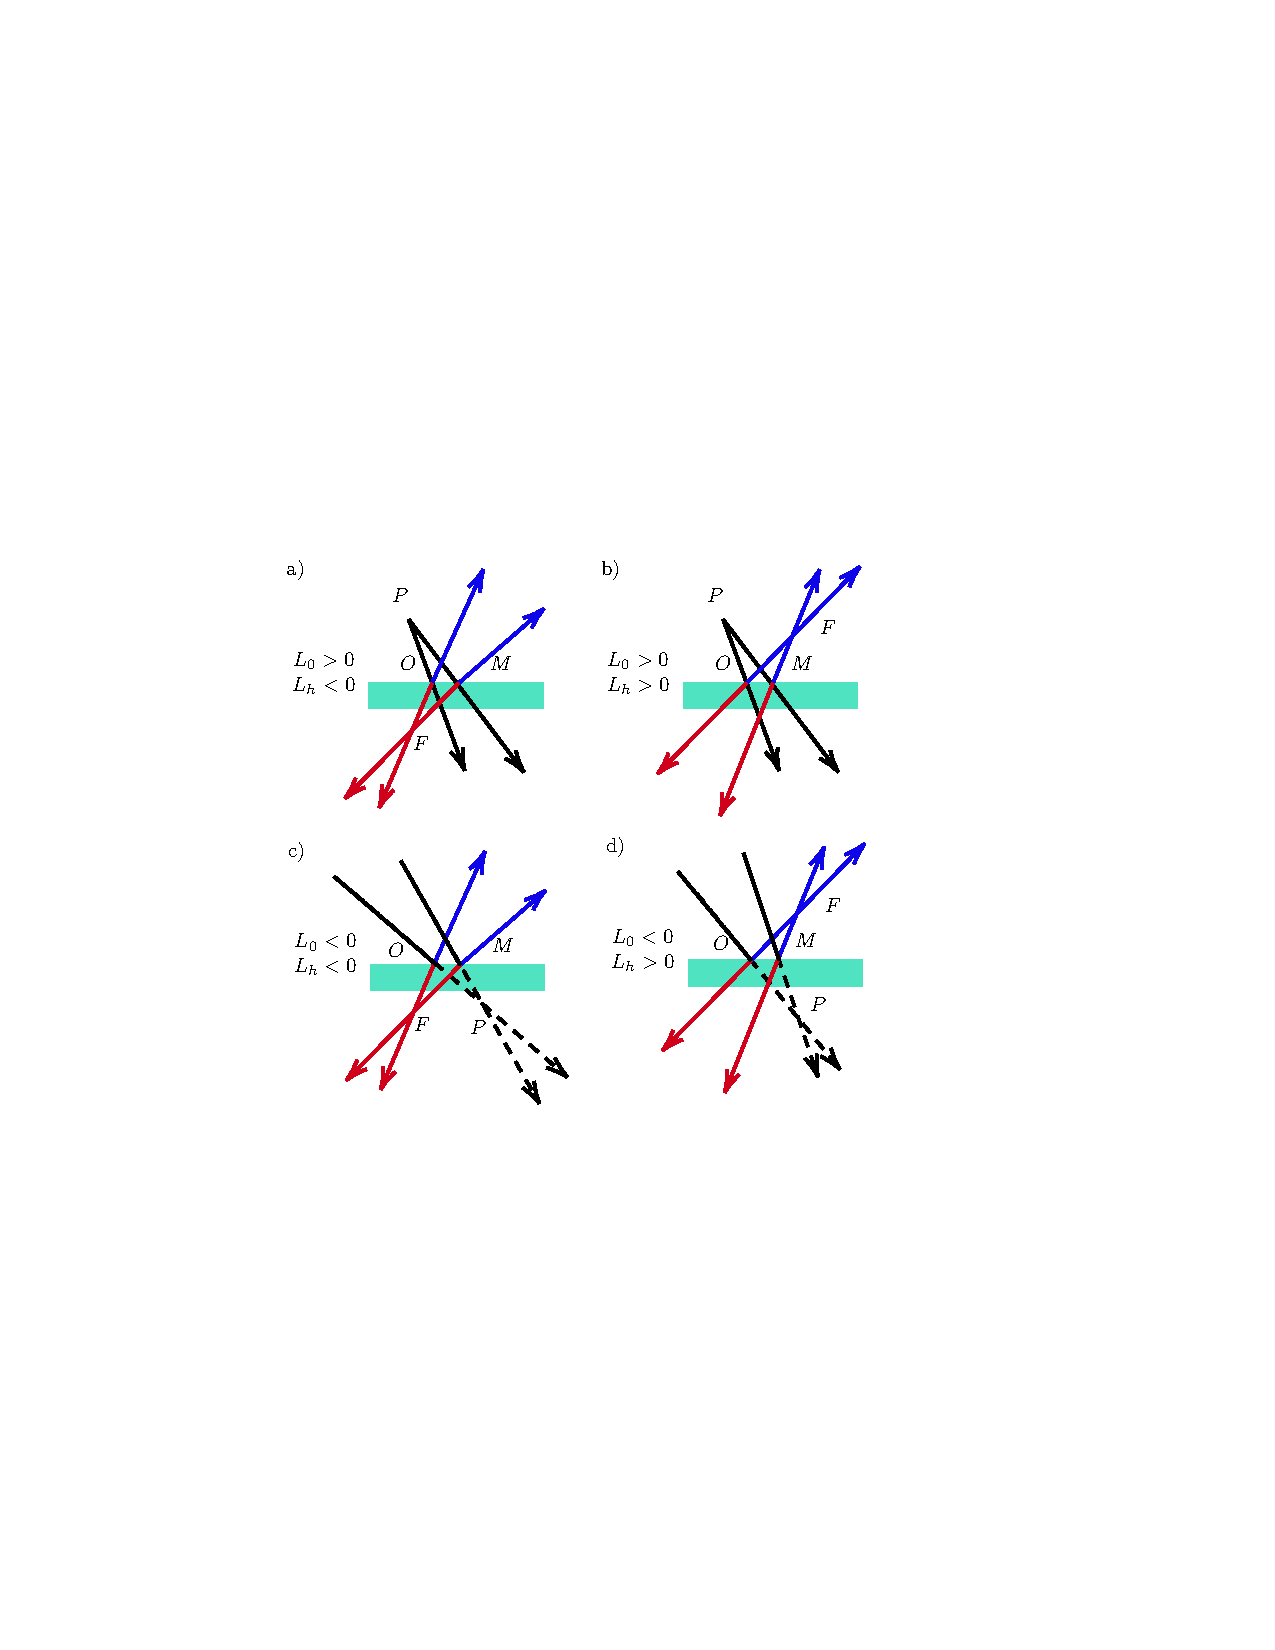
\includegraphics[width=0.99\textwidth,trim=4cm 9cm 6cm 9cm,clip=true]{fig1.pdf}
\end{figure}

Consider a monochromatic x-ray or neutron beam emitted by a point-source $S$. The origin of coordinates is chosen at the point $O$ of the crystal surface in such a way that the wave-vector  ${\vec k_0}$ of the central incident ray $\overline{SO}$, is in exact Bragg  position. The diffracted ray has a wave-vector $\vec k_h$ given by the Laue equation $\vec k_h = \vec k_0 + \vec h$, where $\vec h$ is the reciprocal lattice vector (see Fig.~\ref{fig:vectors}). This is valid for both transmission geometry (Laue) or reflection geometry (Bragg). 

We use oriented angles $\varphi_0 = (\vec n, \vec k_0)$ and $\varphi_h = (\vec n, \vec k_h)$, where $\vec n$ is the inward normal to the crystal surface. $\varphi_0$ is positive, without loss of generality; $\theta_B$ is the modulus of the Bragg angle,
% equal to $|\varphi_0-\varphi_h|/2$ in Laue case and  $|\varphi_h-\varphi_0|/2$ in Bragg case.
The special case of symmetric geometry, with asymmetry angle $\alpha=0$, is such that $\varphi_{0,h}=\pm\theta_B$ in Laue or $\varphi_{0,h}=(\pi/2)\mp\theta_B$ in Bragg. Otherwise, the asymmetry angle $\alpha$ is defined as the angle of rotation of the vectors $(\vec h, \vec k_0, \vec k_h)$ from their directions in the symmetrical case. 
% It follows that $\varphi_0+\varphi_h=2\alpha$ in Laue case and  $\varphi_0+\varphi_h=2\alpha+\pi$ in Bragg case.
In Laue case $\varphi_{0,h}=\pm\theta_B+\alpha$; in Bragg case $\varphi_{0,h}=(\pi/2)\mp\theta_B+\alpha$, therefore $2\theta_B=|\varphi_0-\varphi_h|$ in both cases, $2\alpha=\varphi_0+\varphi_h$ in Laue case and $2\alpha=\varphi_0+\varphi_h-\pi$ in Bragg case.

When moving the point of incidence over an arbitrary small distance $s$ along the curved crystal surface (see Fig.~\ref{fig:vectors}), 
$\vec k_{0,h}$ are changed in direction (not in module), with rotation angles $\epsilon_{0,h} = (\vec k_{0,h},\vec k'_{0,h})$; $\vec h$ and $\vec n$ are changed into $\vec h'$ and $\vec n'$, respectively, due to the crystal bending;
$\varphi_{0,h}$ are changed into $\varphi'_{0,h}=\varphi_{0,h}+\Delta \varphi_{0,h}$.
The projections of the vectors $\vec k'_{h}$ and $\vec k'_{0}+\vec h'$ on the crystal surface are equal, as a result of the conservation of the parallel components of wave-vectors. The surface projections of $\vec k'_{0,h}$ 
are equal to $k \sin\varphi'_{0,h}$. Furthermore, in the present case of cylindrical bending, the surface projections of $\vec h'$ is constant (the angle between the $\vec h$ and $\vec n$ is constant).
This implies that $(\sin \varphi'_h - \sin \varphi'_0) = (\sin \varphi_h - \sin \varphi_0)$ is invariant, therefore
\begin{equation}
\label{eq:invariant}
    \Delta \varphi_h \cos\varphi_h = \Delta \varphi_0 \cos\varphi_0.
\end{equation}

\begin{figure}
\label{fig:vectors}
\caption{Schematic view of the relevant parameters in focusing by a bent crystal in Bragg geometry.
}
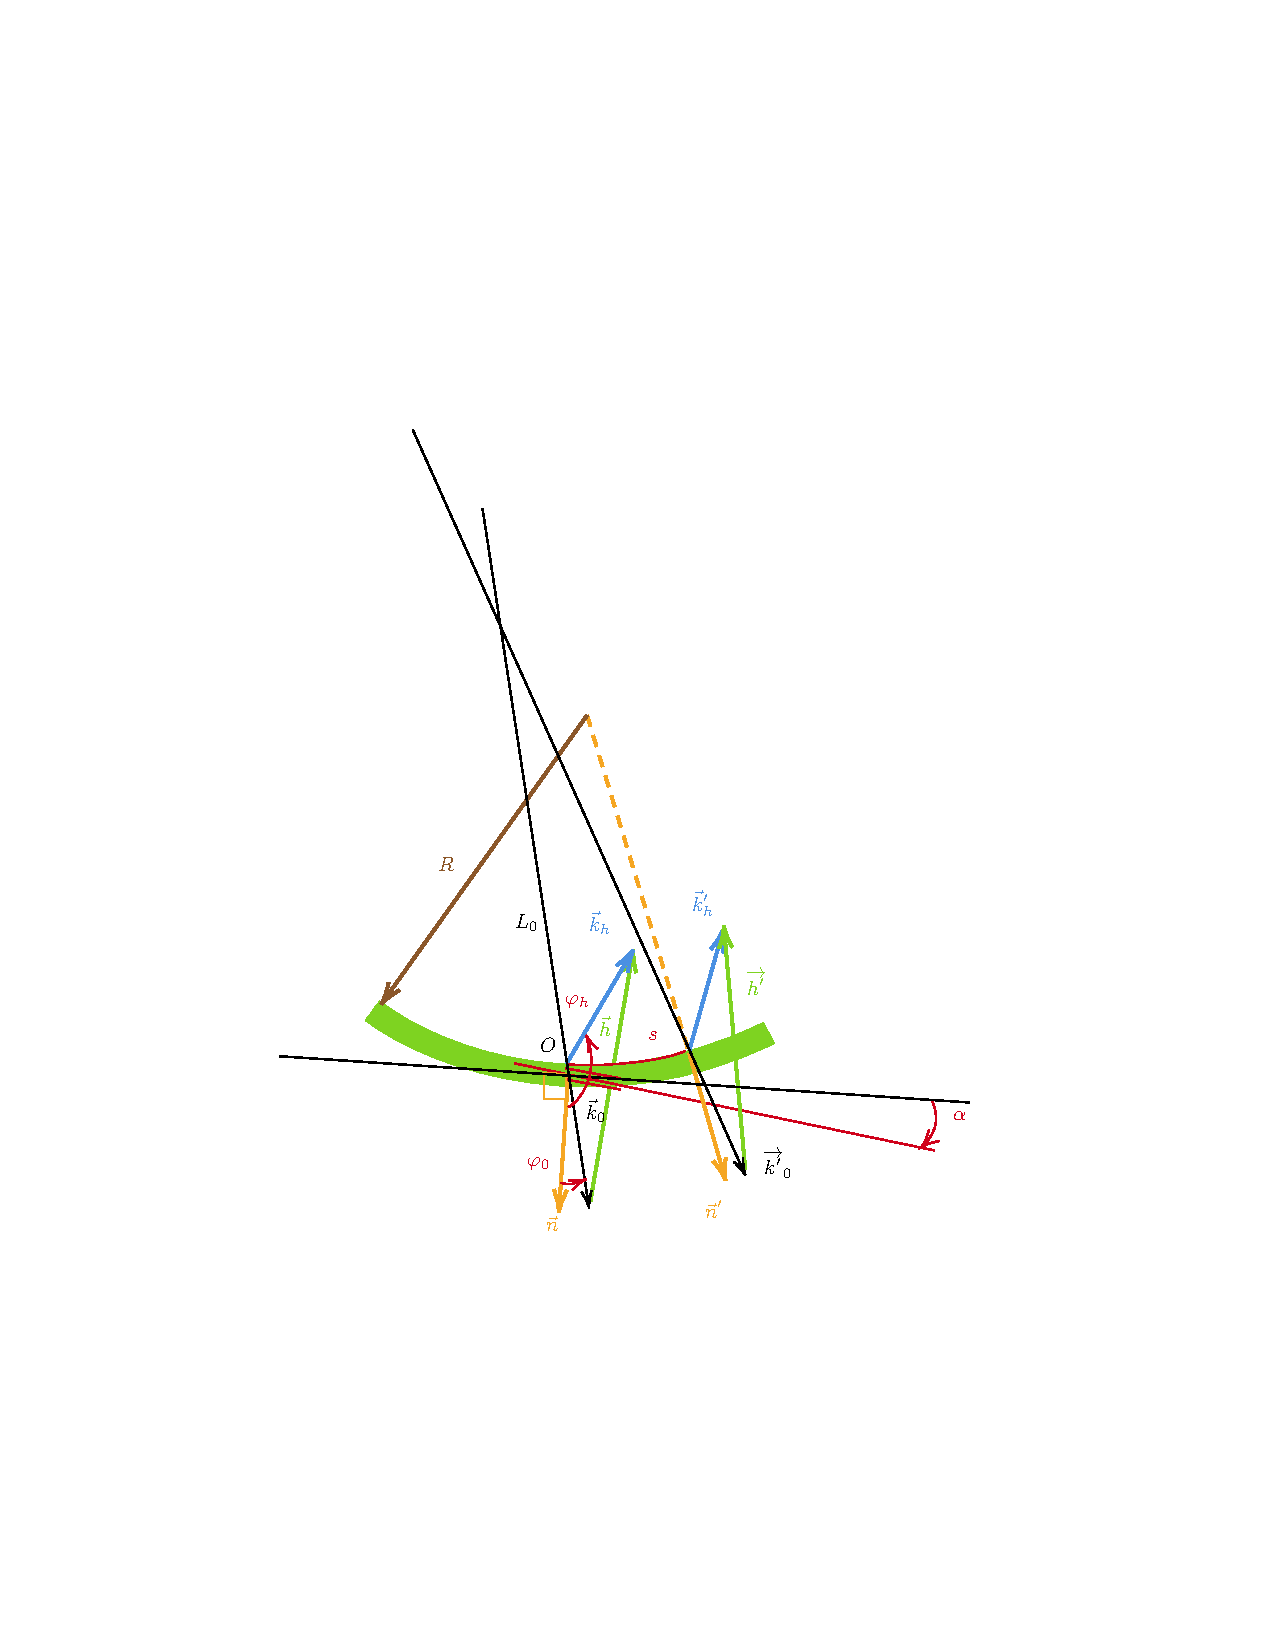
\includegraphics[width=0.99\textwidth,trim=4cm 6cm 5cm 10cm,clip=true]{fig2.pdf}
\end{figure}

The source distance $L_0=\overline{SO}$ is set as positive if the source is on the incidence side of the crystal (real source) or negative if the source is on the other side (virtual source) (see Fig.~\ref{fig:geometries}). The radius of curvature $R_c$ is set as positive if the x-ray beam is incident on the concave side of the bent crystal surface. The focus distance $L_h$ is set as positive if the real or virtual focus is situated on the incidence side on the crystal. With these conventions, $(\vec n,\vec n')=s/R_c$, $\epsilon_0 L_0 = s \cos\varphi_0$,  $\epsilon_h L_h = s |\cos\varphi_h|$. Using the relationship
\begin{equation}
    \varphi'_{0,h} = 
    (n',  \vec k'_{0,h}) = 
    (\vec n', \vec n) + (\vec n,\vec k_{0,h}) + (\vec k_{0,h}, \vec k'_{0,h}) = -\frac{s}{R_c} + \varphi_{0,h} + \epsilon_{0,h},
\end{equation}
we obtain

\begin{equation}
\label{eq:angles}
\Delta \varphi_0 =  - \frac{s}{R_c} + s \frac{\cos\varphi_0}{L_0}
\end{equation}
and 
\begin{equation}
\label{eq:angles2}
\Delta \varphi_h = - \frac{s}{R_c} +  s \frac{|\cos\varphi_h|}{L_h}.
\end{equation}

The crystal lens equation is finally obtained by inserting these expressions in equation~(\ref{eq:invariant})

\begin{equation}
\label{eq:CLE}
\frac{|\cos\varphi_h| \cos\varphi_0}{L_h} - \frac{\cos^2\varphi_0}{L_0} = \frac{\cos\varphi_h - \cos\varphi_0}{R_c}.
\end{equation}


Equation~\ref{eq:CLE} is valid in both Bragg and Laue cases. In the Laue symmetrical case ($\cos\varphi_h=\cos\varphi_0$) it predicts $L_h=L_0$(for a real source, the focus is virtual at the same distance than the source) and, in the particular case of $L_0=+\infty$, a plane incident wave is diffracted into a plane wave.

The crystal lens equation~(\ref{eq:CLE}) obtained here is different from the equation given in \cite{CK}\footnote{The CLE in \cite{CK} is 
$
\cos\varphi_h |\cos\varphi_0|/L_h + \cos^2\varphi_0/L_0 = (\cos\varphi_0 + \cos\varphi_h)/R 
$}. Both equations are equivalent for the Bragg case ($\cos\varphi_h<0$), but not for the Laue case.

Equation~\ref{eq:CLE} is obtained here using a geometrical ray optics approach. It can also be deduced from a wave-optics approach as shown in Appendix~\ref{appendix:CLE}. 

It is worth mentioning that the lens equation~(\ref{eq:CLE}) discussed here can be applied only for monochromatic radiation. Polychromatic focusing is discussed in section~\ref{sec:polychromatic} in the more general context of dynamical theory of diffraction.

Note that we used in this section the same notation as \cite{CK}, where $R_c$ is positive for a concave surface, used to focus in Bragg case. For the rest of the paper, we choose the notation: $p \leftarrow L_0$, $q \leftarrow -L_h$ $R \leftarrow -R_c$, $\theta_1 \leftarrow \varphi_0$ and $\theta_2 \leftarrow \varphi_h$.
This notation is commonly used for Laue crystals, because real focusing is obtained when the beam coming from a real source is incident on the convex side of the bent crystal (with positive $R$).

\section{Dynamical focusing in Laue geometry}
\label{sec:dynamlicalLaue}

The applicability of the CLE for the Laue case is very limited. The results predicted by CLE ignore dynamical effects that must be taken into account in a realistic view of the beam evolution after diffraction by a Laue crystal. The dynamical theory of diffraction predicts ``new" focal conditions, even for flat Laue crystals, that are relevant in experiments and are not explained by the simple CLE. We analyze here the propagation of x-rays by Laue crystals in the framework of the dynamical theory of diffraction (see book \cite{authierbook} \todo{CHECK YEAR}), and propagation in free space is based on paraxial wave optics. 

% \todo{MOVED LATER (SECTION 3.2)}\sout{
% The incident wave-amplitude is expressed in a plane perpendicular to the incidence direction at a negligible distance from the entrance surface (axis $\tau$ in Fig.~\ref{fig:laue}).
% Similarly, we will express the Bragg-diffracted amplitude $D_h$ in a plane perpendicular to the direction of the Bragg diffraction at a negligible distance from the exit surface (axis $\xi$ in Fig.~\ref{fig:laue}).}

% \todo{AN OLD PARAGRAPH IS DISTRIBUTED AMONG THE SUBSECTIONS. WHERE TO PUT CITE \cite{kushnir}??? ALSO THIS IS NOT SAID: Wave propagation in free space is based on paraxial wave optics.
% }


\subsection{Influence function derived from the Takagi-Taupin equations}
\label{sec:influence}


We introduce the Takagi-Taupin equations and the influence functions representing the wavefield for a point-source on the crystal entrance surface. The x-ray wavefield inside the crystal is expressed as the sum of two modulated plane waves
\begin{equation}
    \Psi(\vec x) = D_0(\vec x) e^{i \vec k_0 . \vec x} + D_h(\vec x) e^{i \vec k_h . \vec x},
\end{equation}
with slowly varying amplitudes $D_{0,h}(\vec x)$.
The spatial position $\vec x$ is expressed in oblique coordinates $(s_0,s_h)$ along the directions of the $\vec k_0$ and $\vec k_h=\vec k_0 + \vec h$ vectors.
% The incident wave is also expressed as a modulated plane wave $D_{inc}(\vec x) \exp(i\vec k_k . \vec x)$. 
The differential Takagi-Taupin equations  \cite{Takagi1962, Takagi, Taupin, Taupin1967}, hereafter referred to as TTE, are
\begin{subequations}
\label{eq:TT}
\begin{align}
\frac{\partial D_0}{\partial s_0} =& \frac{ik}{2} \left[ \chi_0 D_0(\vec x)+c \chi_{\bar h} e^{i \vec h . \vec u (\vec x)} D_h(\vec x) \right]; \\
\frac{\partial D_h}{\partial s_h} =& \frac{ik}{2} \left[ \chi_0 D_h(\vec x)+c \chi_{h} e^{-i \vec h . \vec u (\vec x)} D_0(\vec x) \right],
\end{align}
\end{subequations}
where $k=2\pi/\lambda=|\vec k_0|=|\vec k_h|$; $\chi_0$, $\chi_h$, and $\chi_{\bar h}$ are the Fourier coefficients of order 0, $\vec h$ and $-\vec h$ of the undeformed crystal polarisability. The polarization factor $c$ ($c=1$ for $\sigma$-polarization and $c=\cos2\theta_B$  for $\pi$-polarization) will be omitted afterwards, for simplicity. 
In the equations~(\ref{eq:TT}), $\vec u (\vec x)$ is the dispacement field of the deformed crystal.
% The ``influence functions", hereafter called IF, are the solutions of the TT equations corresponding to a point source in the crystal entrance surface.
In the case of a cylindrically bent crystal, the deformation phase factor is of the form
\begin{equation}
\label{eq:cylinder}
    \vec h . \vec u = -A s_0 s_h + \phi_1(s_0) - \phi_2(s_h)
\end{equation}
where $A$ and the $\phi_{1,2}$ functions are explicited in Appendix~\ref{appendix:Deformation}.
Equation~(\ref{eq:cylinder}) corresponds to the case of a ``constant strain gradient" \cite{authierbook} meaning that $\partial^2(\vec h . \vec u)/(\partial s_0 \partial s_h)$ is constant.
\inblue{It is \inred{useful} to introduce the functions $G_{0,h}(s_0,s_h)$ defined by
  \begin{subequations}
    \label{eq:functionsG}
    \begin{align}
      D_0(s_0,s_h) &= G_0(s_0,s_h) \exp[i\frac{k}{2}\chi_0 (s_0+s_h)-i \phi_2(s_h)\\
      D_h(s_0,s_h) &= G_h(s_0,s_h) \exp[i\frac{k}{2}\chi_0 (s_0+s_h)-i \phi_1(s_0)+iAs_0s_h]
    \end{align}
  \end{subequations}

for which TTE have a simpler form
  \begin{subequations}
    \label{eq:TTEsimple}
    \begin{align}
      \frac{\partial G_0}{\partial s_0} &= i \frac{k}{2}\chi_{\bar{h}} G_h
      \\
      \frac{\partial G_h}{\partial s_h} &= i \frac{k}{2}\chi_{\bar{h}} G_0 - i A s_0 G_h
    \end{align}
  \end{subequations}

An incident monochromatic wave of any form can also be expressed as a modulated plane wave $D_{inc}(\vec x)\exp(i \vec k_0 . \vec x)$ defining a continuous distribution of coherent elementary point-sources on the crystal surface, according to the general Huyghens principle in optics. The “influence functions” (or propagators), hereafter refered to as IF, are the TTE solutions corresponding to these point-sources. The IF for a point-source of  oblique coordinates $(\sigma_0,\sigma_h)$, in the case of  a crystal with deformation that verifies equation~(\ref{eq:cylinder}), are derived in \cite{GuigayFerrero2016} by formulating the TTE  as integral equations in the case of an incident wave of the form. The calculations are presented in appendix~\ref{appendix:TTEintegral},} \inred{result in a diffracted electric field}\footnote{the result for the transmitted amplitude $D_0(s_0,s_h)$ is not necessary for our results and is not presented here, but it is easily obtained using equation~(\ref{eq:kummer}) in (\ref{eq:TTEsimple}).}
% An incident monochromatic wave of any form, can also be expressed as a modulated plane wave $D_{inc}(\vec x)\exp(i\vec k_0. \vec x)$ defining a continuous distribution of coherent point-sources on the crystal surface, according to the general Huyghens principle in optics. The influence functions, or propagators, are the solutions of the TTE corresponding to these point-sources. The IF for a point-source of coordinates $(\sigma_0,\sigma_h)$, in the case of crystals with deformation that verify equation~(\ref{eq:cylinder}), are derived in \cite{GuigayFerrero2016} by formulating the TTE as integral equations and solving them by iteration, starting from the undiffracted term $D_{inc}(s_0,s_h\inred{;\sigma_0,\sigma_h})=\exp[ik(s_0-\sigma_0)]\delta(s_h-\sigma_h)$, with $\delta$ the Dirac delta. The result for the diffracted field $D_h$ is
% \begin{multline}
% \label{eq:preKummer}
%     D_h(s_0,s_h) =  \frac{i k}{2} \chi_h e^{(ik/2) \chi_0 (s'_0 + s'_h)} e^{i A s'_o s'_h - i\vec h.\vec u(s_o,\sigma_h)} \times
%     \\
%     [1 + \sum_{i=1}^\infty \frac{(\Omega + i A )(\Omega+2iA)...(\Omega+niA)}{n!n!}(-s'_0s'_h)^n],
% \end{multline}
% where $s'_{0,h}=s_{0,h}-\sigma_{0,h}$ and $\Omega = k^2 \chi_h \chi_{\bar h}/4$. The first exponential stands for the effects of refraction and normal absorption. For $A\ne0$, the equation~(\ref{eq:preKummer}) can be expressed as
  
\begin{equation}
\label{eq:kummer}
    D_h(s_0,s_h) = \frac{i k }{2} \chi_h e^{(ik/2) \chi_0 (s'_0 + s'_h)} e^{i \vec h . \vec u (s_0,\sigma_h)} M(\frac{i\Omega}{A},1,iA s'_0 s'_h)
\end{equation}
where the the first exponential term stands for the effect of refraction and normal absorption, $s'_{0,h}=s_{0,h}-\sigma_{0,h}$, $\Omega=k^2\chi_h\chi_{\bar{h}}/4$ and the $M$ function is known as the Kummer function (a confluent hypergeometric function) defined by the convergent infinite series
\begin{equation}
\label{eq:kummerSeries}
    M(a,b,z) = 1 + \frac{a}{b} z + 
    ... + \frac{a(a+1)...(a+n-1)}{n! b (b+1)...(b+n-1)}z^n+...
\end{equation}

This type of solution of the TTE was already obtained a long time ago, by different methods \cite{Petrashen1974,Katagawa1974,Litzmann1974,Chukhovski1977}.

The exponential term $\exp(i \vec k . \vec h(s_0,\sigma_h))$ in equation~(\ref{eq:kummer}) is the phase shift acquired at the scattering event occurring at the point of oblique coordinates $(s_0,\sigma_h)$along the ray incident in the point $(\sigma_0,\sigma_h)$. It therefore represents the kinematical (single-scattering) approximation of the dynamical theory.

In the case of $A=0$, the Kummer function in equation~(\ref{eq:kummer}) reduces to the Bessel function $J_0(2\sqrt{\Omega s'_0 s'_h})$. 
          
\subsection{Dynamical focusing and Borrmann effect in a flat crystal plate in general Laue geometry}
\label{sec:LaueFlat}


\todo{VERIFY ALL THIS SECTION}


This section introduces the important case of dynamical focusing with flat Laue crystals (without bending), first described in \cite{AfanasevKohn1977} and verified experimentally by \cite{Aristov1978, Aristov1980}
in the case of symmetrical geometry. The theory was extended to the asymmetric case by \cite{Kohn2000}. The dynamical diffraction focusing by a system of two Laue crystals was recently considered by \cite{KohnSmirnova}. Diffraction focusing by a system of two identical perfect Laue crystals was previously applied to neutron interferometry \cite{Zeilinger}.
\todo{CHECK REF Zeilinger}


\begin{figure}
\label{fig:laue}
\caption{Schematic representation of the relevant parameters in Laue asymmetrical diffraction.
}
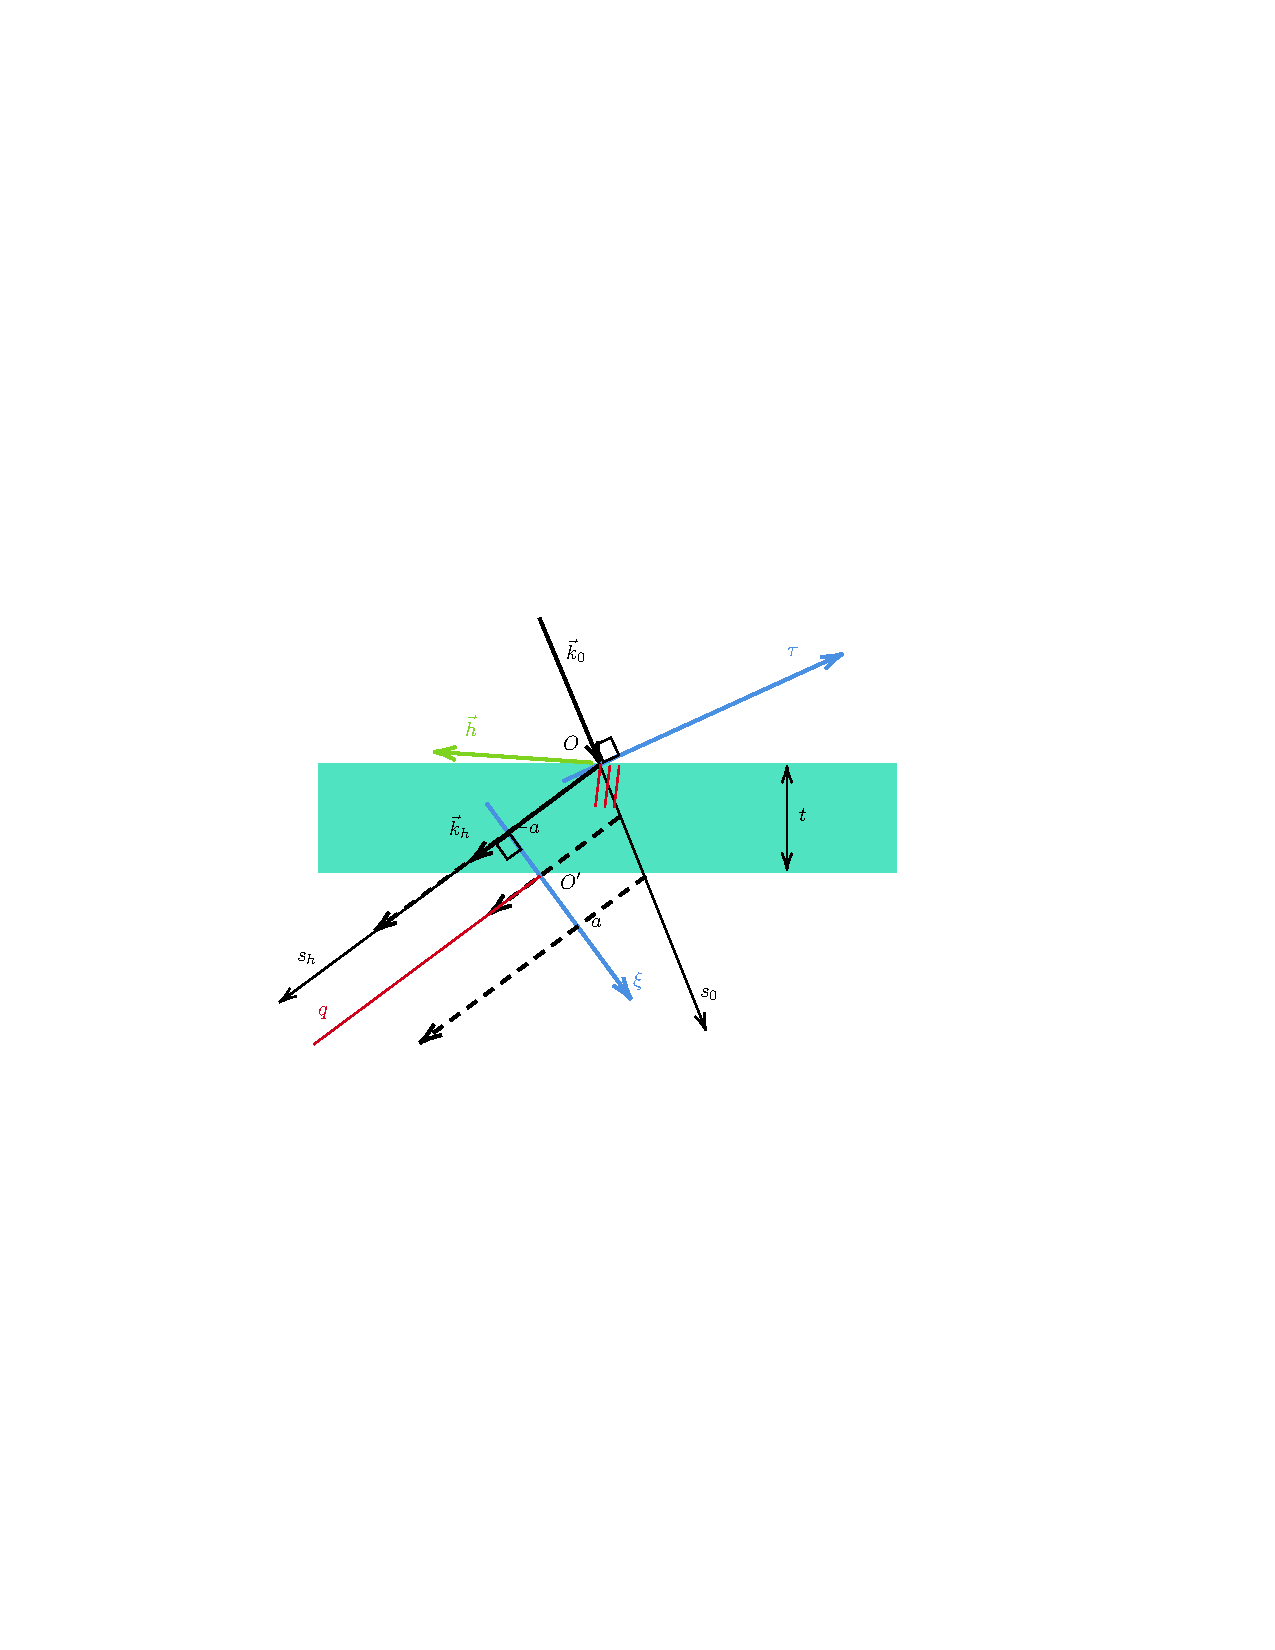
\includegraphics[width=0.99\textwidth,trim=3cm 10cm 5cm 10cm,clip=true]{fig3.pdf}
\end{figure}

% The incident wave-amplitude is expressed in a plane perpendicular to the incidence direction at a negligible distance from the entrance surface (axis $\tau$ in Fig.~\ref{fig:laue}).
% Similarly, we will express the Bragg-diffracted amplitude $D_h$ in a plane perpendicular to the direction of the Bragg diffraction at a negligible distance from the exit surface (axis $\xi$ in Fig.~\ref{fig:laue}). 
% The dynamical focusing is most easily described by considering a point-source on the crystal entrance surface (in practice, a slit of negligible width placed near the crystal surface).

\inblue{We consider a point-source of coordinates $\sigma_0=\sigma_h=0$ on the crystal entrance surface (in practice, a slit of negligible width placed near the crystal surface). This is the most basic case of dynamial focusing. 

To a point in the $\xi-$axis perpendicular to the direction of $\vec k_h$ and at negligible distance from the crystal of thickness $t$ (see Fig.~\ref{fig:laue}), corresponds to a point of oblique coordinates  $(s_\inred{0},s_h)=((a+\xi)/\sin2\theta_B,\gamma(a-\xi)/\sin2\theta_B)$ on the crystal exit surface, with $a=t \sin2\theta_B/(2\cos\inred{\theta_1})$ and $\gamma=\cos\inred{\theta_1}/\cos\inred{\theta_2}$ (asymmetry ratio). 
}

The reflected amplitude $D_h(\xi)$, is zero outside the interval $-a<\xi<a$, with $a=t \sin2\theta_B/(2 \cos\inred{\theta_1})$, and it is proportional to the zeroth-order Bessel function  $J_0(Z\sqrt{a^2-\xi^2})$ in this interval \inblue{\cite{kato1961}}, with  $Z=k\sqrt{\gamma\chi_h\chi_{\bar h}}/\sin2\theta_B$. In the case $|Z a| \gg 1$ the asymptotic approximation
\begin{equation}
    J_0(Z\sqrt{a^2-\xi^2})\approx \left(\frac{2}{\pi Z \sqrt{a^2-\xi^2}}\right)^{1/2} \cos(Z\sqrt{a^2-\xi^2}-\pi/4)
\end{equation}
can be used in the central region $|\xi|\ll a$ where we can also use
\begin{equation}
     \sqrt{a^2-\xi^2} = a (1-\frac{\xi^2}{2a^2}+...)\approx a - \frac{\xi^2}{2a}.
\end{equation}
We thus obtain in this central region the approximation
\begin{equation}
\label{eq:approximatedDiffractedField}
    J_0(Z\sqrt{a^2-\xi^2})\approx \left(\frac{2}{i \pi Z a}\right)^{1/2} \left( e^{iZa-i Z\frac{ \xi^2}{2a}} + i 
    e^{-i Z a+i Z\frac{\xi^2}{2a}} \right),
\end{equation}
where the two exponential terms are related to the two sheets of the dispersion surface. 
If $\operatorname{Re}(Z)>0$ the function $\exp(- i Z \xi^2 / (2 a))$ 
represents a converging wave (divergent if  ($\operatorname{Re}(Z)<0$). A double, real and virtual, focusing effect is thus expected at opposite distances $\pm q_0$ from the crystal, with
\begin{equation}
\label{eq:q0}
    q_0 = \frac{k a}{|\operatorname{Re}(Z)|}= \frac{a \sin2\theta_B}{|\operatorname{Re}(\sqrt{\chi_h\chi_{\bar h}})|}
\end{equation}

The parameter $q_0$, which may be referred to as the ``dynamical approximated focal length", depends on the asymmetry angle through the half-width a of the Bragg-diffracted beam $a$. It gives the position of the beam waist only approximately, as several approximations have been used.

The reflected amplitude at any distance $q$ from the crystal can be calculated numerically, without the approximations used above, by propagating the wavefield at the crystal exit
\begin{equation}
    D_h(\xi,0)=i \frac{k}{2}\chi_h J_0(Z\sqrt{a^2-\xi^2})
\end{equation}
via convolution with the Fresnel propagator:
\begin{equation}
\label{eq:Fresnel}
    D_h(\xi; q) = (\lambda q)^{-1/2} \int_{-a}^a d\xi'  \, e^{i k 
    \frac{(\xi-\xi')^2}{2 q}} 
    D_h(\xi',0).
\end{equation}
The resulting ``axial intensity profile" $|D_h(0,q)|^2$ shows in general two strong maxima at distances $q_{1,2}=\pm q_{dyn} < q_0$. This difference is a cylindrical aberration effect related to the approximations used to obtain equation (\ref{eq:q0}). The parameter $q_{dyn}$ is the ``dynamical focal length" obtained numerically, thus non-approximated (contrary to $q_0$). Note that $q_0$ is exactly proportional to the crystal thickness \inred{but this is not true for $q_{dyn}$}. As an example, some numerical values are given in Table~\ref{table:example}.
\inred{It can be appreciated a difference in the absolute value of $q_{dyn}$ for the negative and positive values. This is due to absorption. Without absorption, $D_h$ in equation~(\ref{eq:Fresnel}) would be real, giving the same absolute value. Because $D_h$ is complex, the $q_{dyn}$ values are slightly different for the positive and negative directions, as shown in Fig.~\ref{fig:flatLaue}}


% photon_energy_in_keV: 8.3
% >>>>>>>>>> after teta_deg: 13.781015282157512
% >>>>>>>>>> after chizero: (-1.4243708572190367e-05+3.1690484405626266e-07j)
% >>>>>>>>>> chih: (-5.5485418686499844e-06-5.231637024593725e-06j)
% >>>>>>>>>> lambda1: 1.4937855232915694e-07
% raygam 971.2132636651617
% attsym 0.03234813288425055
% asym,halfwith of reflected beam 0.05955291579808722
% zasym (41.266534622241025-1.2131120316936161j)
% qzero, dynamical focal length 3614.928251103722
% qpoly, polychromatic focal distance 480.93572032706084
% pe 952.7076181620846
% File written to disk: mypoints1_8keV_positive.txt
% Maxumum found at x=2861.86, y=0.0226271

% photon_energy_in_keV: 17.0
% >>>>>>>>>> after teta_deg: 6.6788054915157336
% >>>>>>>>>> after chizero: (-3.3571064151915308e-06+1.8177082932893733e-08j)
% >>>>>>>>>> chih: (-1.2748345525524618e-06-1.2566574696195692e-06j)
% >>>>>>>>>> lambda1: 7.293188143129426e-08
% raygam 993.2137397205423
% attsym 0.6742392040644324
% asym,halfwith of reflected beam 0.02907583536024259
% zasym (19.408470444960464-0.13936025623969706j)
% qzero, dynamical focal length 3752.628240968803
% qpoly, polychromatic focal distance 491.72300936984254
% pe 973.8685472836659
% File written to disk: mypoints1_17keV_positive.txt
% Maxumum found at x=2559.16, y=0.130538

\begin{table}
\caption{Parameters for symmetrical Laue silicon crystal in 111 reflection and thickness $t$~= \SI{250}{\micro\meter}. Note that $\chi_{\bar h}=-i\chi_h$.}
\begin{tabular}{lcccccc}
 Photon \\energy  [keV]  & $\theta_B$ [deg]       & $\chi_0$ & $\chi_h$ & $a$ [\SI{}{\micro\meter}]& $q_0$ [mm] & $q_{dyn}$  [mm] \\
\hline
 8.3  &  13.78 & -1.42e-5+3.17e-7i & -5.55e-6-5.23e-6i  & 59  & 3615  & \inred{-2617,}2862   \\
 17   &  6.68 & -3.36e-6+1.82e-8i & -1.27e-6-1.26e-6i  & 29  & 3753  & \inred{-2521,}2559 
\end{tabular}
\label{table:example}
\end{table}


\begin{figure}
\label{fig:flatLaue}
\caption{Numerical evaluation of on-axis intensity for a  \SI{250}{\micro\meter} thick flat Si111 crystal ($R=\infty$) with source at the crystal entrance surface ($p=0$) calculated using equation~(\ref{eq:Fresnel}).
a) Simulation for a photon energy of 8.3 keV.
b) Simulation for a photon energy of 17 keV.
Numerical values of these simulations are in Table~\ref{table:example}. \todo{add numerical constant in ordinates}
}
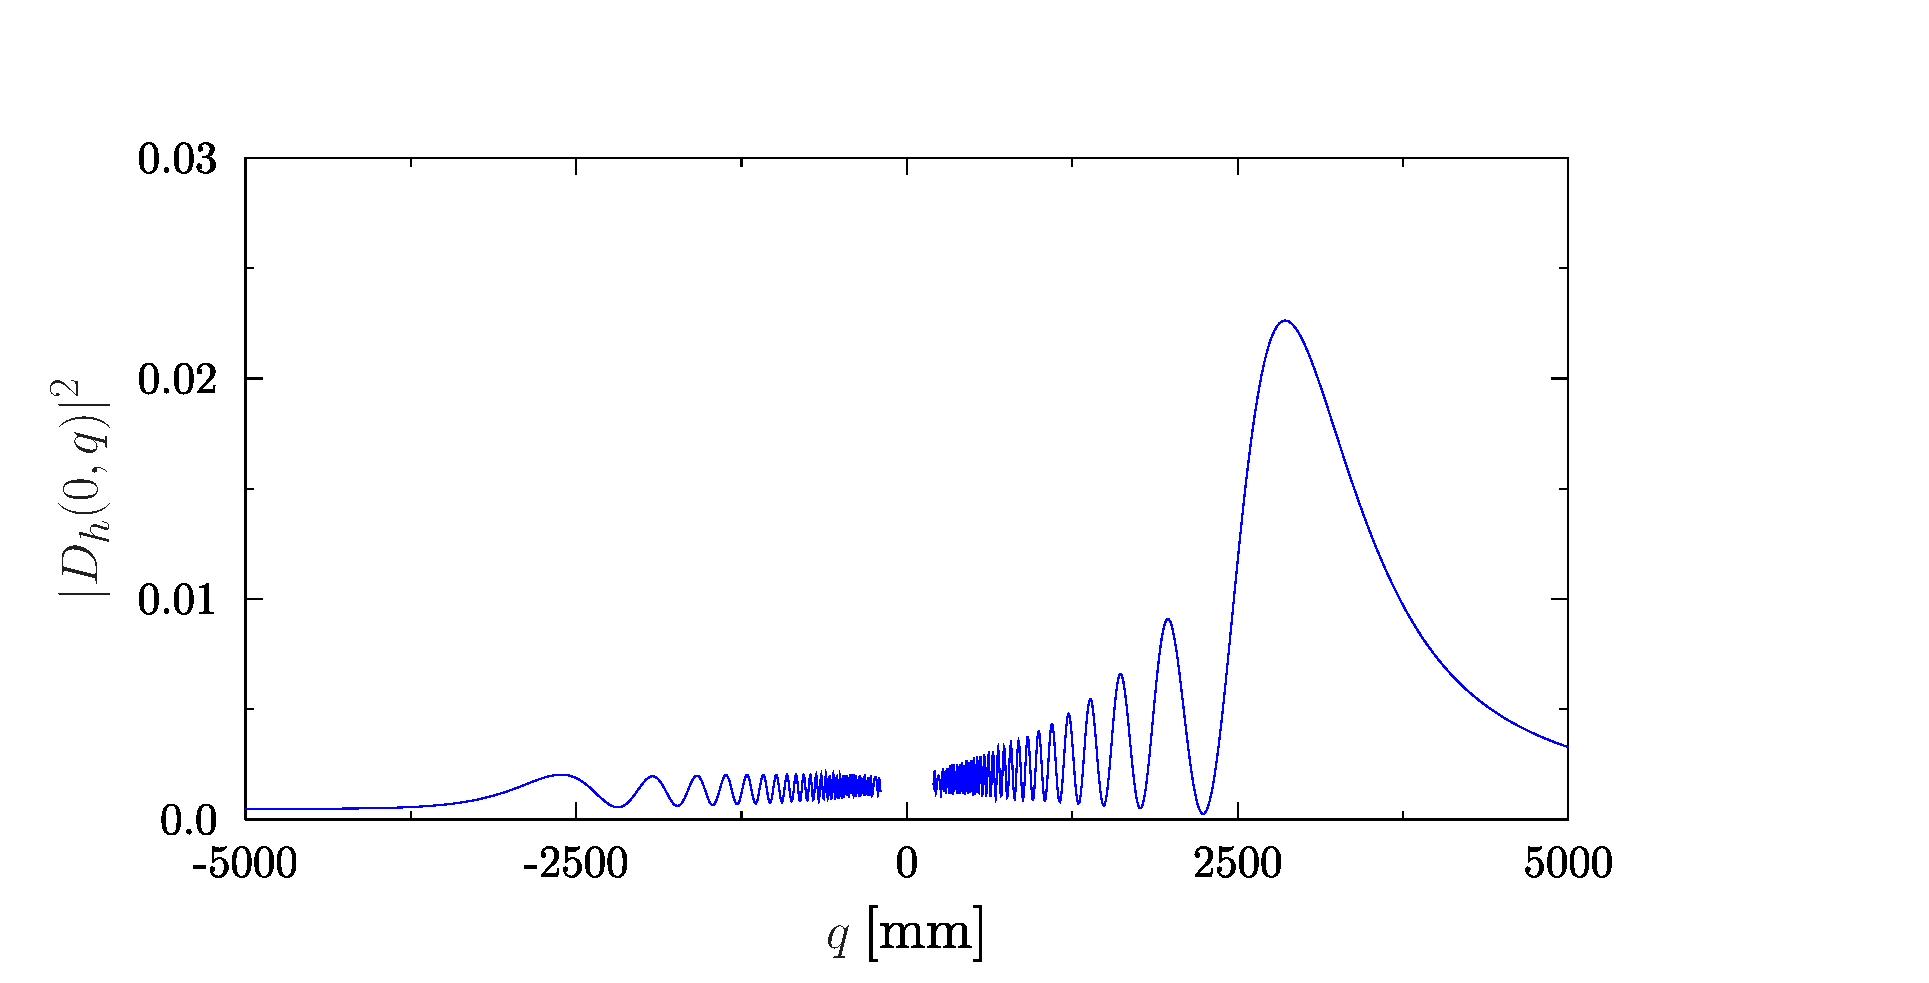
\includegraphics[width=0.95\textwidth]{flat8keV.eps}
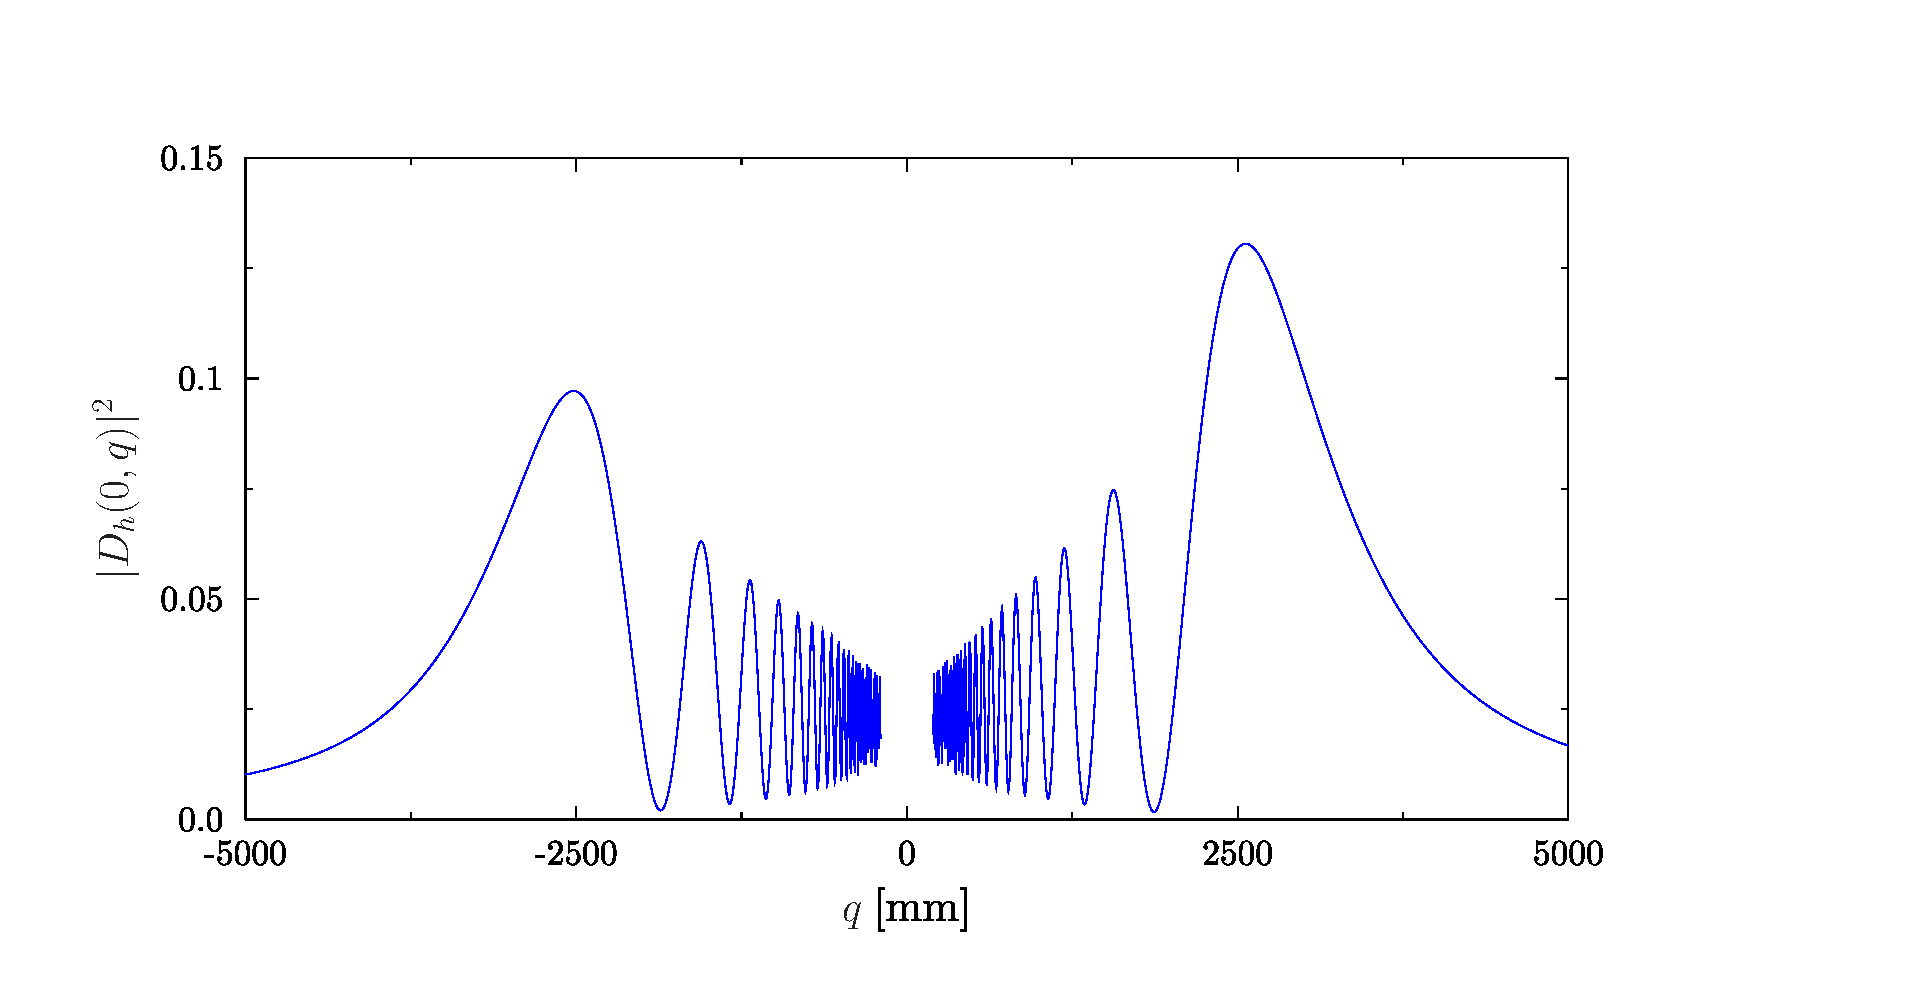
\includegraphics[width=0.95\textwidth]{flat17keV.eps}
\end{figure}

The moduli of the two terms in equation~(\ref{eq:approximatedDiffractedField}) are in general different: they are proportional to $\exp(\mp a \operatorname{Im}(Z))$. This is the expression of anomalous absorption (Borrmann effect). Two focusing positions are to be observed in the case of small absorption; but only one focusing position is to be observed in the case of strong absorption (see Fig.~\ref{fig:flatLaue}). It turns out that this property is also valid if the crystal plate is not flat, but cylindrically bent around an axis normal to the diffraction plane. 

For the flat crystal under discussion, the focusing condition for a source at a finite distance $p$ from the crystal, is 
\begin{equation}
    \label{eq:sumpandq}
    p+q=\pm q_{dyn}.
\end{equation}
This result is simply obtained by looking at the operators i) the free-space propagation from the source to the diffracting crystal, ii) effect of the crystal diffraction, and iii) the propagation downstream from the crystal to the image position. These operations  are space-invariant. They are expressed as convolutions in direct space, or simply multiplications in reciprocal space. Therefore, they can be commuted. This allows to merge the operations i) and iii) and consequently obtain equation~(\ref{eq:sumpandq}).
Propagation through a flat crystal is space-invariant, whereas propagation through a bent crystal is not space-invariant. The reason for this difference is that, in a bent crystal case, the IF is not only dependent on the variables $(s'_0,s'_h)$, but also on the variables $(\sigma_0,\sigma_h)$, as seen in equations~(\ref{eq:TTEsimple},\ref{eq:kummer}).



\subsection{Lens equation for a bent crystal of finite thickness in symmetrical Laue geometry}
\label{sec:LaueNewCLE}

The equations of dynamical focusing by a bent Laue crystal in symmetrical geometry used by \cite{GuigayFerrero2016} are briefly recalled in this section.

For the case of symmetrical diffraction, the factor $\exp(i \chi_0(s'_0+s'_h))$ \inred{in equation~(\ref{eq:kummer})} is constant and will be omitted.
%, and $A=0$, and the functions $\varphi_1(s_0)$, $\varphi_2(s_h)$, in equation (\ref{eq:cylinder}) are the same function, \inred{written now without subindices}, $\varphi(s_0)$, $\varphi(s_h)$}. 
The equation~(\ref{eq:kummer}) can be written as
\begin{equation}
\label{eq:DhSymmetricalLaue}
    D_h(s_0,s_h) = \frac{i k}{2} \chi_h e^{i \vec h . \vec u(s_0,\sigma_h)}
    J_0(2\sqrt{\Omega s'_0 s'_h}),
\end{equation}
with 
\begin{equation}
\vec h . \vec u (s_0,\sigma_h) = \phi(\sigma_h)-\phi(s_0) =
k \frac{\tau(\tau+a)-\xi(\xi+a)}{2 R \cos\theta_B}, 
\end{equation}
$s_0=(\xi+  a)/\sin2\theta_B$,
$\sigma_h=-\tau/\sin2\theta_B$, and
\begin{equation}
\phi(s_0)=\frac{k \sin\theta_B}{R}(s_0^2 \sin2\theta_B - a s_0)=k \frac{\xi(a+\xi)}{2R\cos\theta_B}. 
\end{equation}

Let us consider the incident wave amplitude $D_{inc}(\tau)=\exp(i k \tau^2/(2p))$, where $\tau$ is a coordinate along the axis $O\tau$ normal to $\vec k_0$ (see Fig.~\ref{fig:laue}). The diffracted wave on the axis $O\xi$
($q=0$) is

\begin{equation}
    D_h(\xi,0)=\int_{\xi-a}^{\xi+a}\frac{d\tau}{\sqrt{\lambda p}}
    e^{ik\left[\frac{\tau^2}{2p}+\frac{\tau(\tau+a)-\xi(\xi+a)}{2R \cos\theta_B}\right]}
    J_0(Z\sqrt{a^2-(\xi-\tau)^2}),
\end{equation}
or making the change of variables $\eta=\xi-\tau$,
\begin{equation}
    D_h(\xi,0)=\int_{-a}^{+a}\frac{d\eta}{\sqrt{\lambda p}}
    e^{\frac{ik}{2}\left[\frac{(\xi-\eta)^2}{p}+\frac{\eta^2-2\eta\xi-a\eta}{R \cos\theta_B}\right]}
    J_0(Z\sqrt{a^2-\eta^2}).
\end{equation}
The wave amplitude at a distance $q$ downstream from the crystal is obtained using equation~(\ref{eq:Fresnel}). We thus have a double integral over $\eta$ and $\xi'$. The $\xi'$ integration can be performed analytically \cite{GuigayFerrero2013}, and it turns out that
\begin{equation}
\label{eq:Dhpropagated}
    D_h(\xi,q)=
    \frac{e^{i k \frac{\xi^2}{2L}}}{\sqrt{\lambda L}}
    \int_{-a}^{+a} d\eta
    e^{\frac{ik}{2}
    [\frac{\eta^2}{L_e}-\eta(
    \frac{2\xi q_e}{q L_e}+
    \frac{a}{R \cos\theta_B}
    )]}
    J_0(Z\sqrt{a^2-\eta^2}),
\end{equation}
where $L=p+q$, $p_e^{-1}=p^{-1}+(R\cos\theta_B)^{-1}$, $q_e^{-1}=q^{-1}-(R\cos\theta_B)^{-1}$ and $L_e=p_e+q_e=\pm q_{dyn}$.
\inred{The focal positions are given by $L_{e}=\pm q_{dyn}$}. Using the notation $R'=R\cos\theta_B$, this can be written as
\begin{equation}
\label{eq:preLaueCLE}
    \frac{R'}{R'-q} - \frac{R'}{R' + p} = \pm \frac{q_{dyn}}{R'}.
\end{equation}
Translating equation~(\ref{eq:preLaueCLE}) in the notation of section~\ref{sec:CLE} ($p \to L_0$, $q \to -L_h$, $R \to -R_c$), we obtain
\begin{equation}
\label{eq:newCLE}
    \frac{1}{L_h-R_c \cos\theta_B} -
    \frac{1}{L_0 - R_c \cos\theta_B} =
    \pm \frac{q_{dyn}}{(R_c \cos\theta_B)^2}.
\end{equation}
If $q_{dyn}$ is set to zero, we obtain $L_h=L_0$, the same result as the ``lens equation"~(\ref{eq:CLE}).
Equation~(\ref{eq:preLaueCLE}) or (\ref{eq:newCLE}) can be considered as a ``modified lens equation" which takes dynamical diffraction effects into account in symmetric Laue geometry.

We have not found a closed expression like equation~(\ref{eq:newCLE}) for the general case of asymmetrical Laue diffraction. However, numerical simulations can be done to obtain the focal positions \cite{GuigayFerrero2016, Nesterets}.

We are often interested in real focusing ($q>0$) of an incident beam from a very distant real source ($p\approx \infty$), for instance in EXAFS beamlines. $q_1$ and $q_2$ are both decreasing functions of $p$. Suppose $0<R'\le q_{dyn}$. When $p$ increases from zero to infinity, $q_1$ decreases from $q_1=R'q_{dyn}/(q_{dyn}+R')$ to $q_1=R'(1-R'/q_{dyn})$. Simultaneously, $q_2$ decreases from $q_2=R'q_{dyn}/(q_{dyn}-R')$ to $q_2=R'(1+R'/q_{dyn})$. For very large $p$-values, we have the simple relation $q_1+q_2\approx 2R'$.

Examples of numerical calculations are shown in Fig.~\ref{fig:8keV}, for the case of the 111 reflection of a \SI{250}{\micro\meter} thick cylindrically bent symmetric Laue silicon crystal, with a curvature radius of $R$~= \SI{1}{\meter}, at a source distance $p$~= \SI{30}{\meter} and for x-ray photon energies of 8.3~keV and 17~keV. 
For both photon energy values, the effective value of $q_{dyn}$ is determined by plotting the axial intensity profile as function of $q$ for the unbent crystal of the same thickness and $p=0$ (Fig.~\ref{fig:flatLaue}). This allows to calculate $q_1$ and $q_2$ as

\begin{subequations}
\label{eq:q1andq2}
\begin{align}
    q_1 &= R' \frac{p(q_{dyn}-R')+q_{dyn}R'}{p q_{dyn}+(q_{dyn}+R')R'} \\
    q_2 &= R' \frac{p(q_{dyn}+R')+q_{dyn}R'}{p q_{dyn}+(q_{dyn}-R')R'}.
\end{align}
\end{subequations}

It can be verified that the results are in perfect agreement with the values shown by the numerical plot of the axial intensity profile.
\inred{
Applying the equations (\ref{eq:q1andq2})  to the cases analyzed in Fig.~\ref{fig:8keV} we get (with $q_{dyn}$=~\SI{2862}{\milli\meter} from Table~\ref{fig:flatLaue})
$q_1$=~\SI{644}{\milli\meter},
$q_2$=~\SI{1303}{\milli\meter}. Relative errors are -1.2\% and -2.1\%, respectively with respect to numerical values in Fig.~\ref{fig:8keV}a. For 17 keV (Fig.~\ref{fig:8keV}b)
$q_1$=~\SI{611}{\milli\meter},
$q_2$=~\SI{1382}{\milli\meter}, therefore the relative errors are -2.24\% and 0.7\%, respectively.}


% \todo{For the case in Fig.~\ref{fig:8keV}, at 8.3 keV we obtained numerically $q_1$=~\SI{652}{\milli\meter},
% $q_2$=~\SI{1330}{\milli\meter} and using equations (\ref{eq:q1andq2})  we get (with $q_{dyn}$=~\SI{2862}{\milli\meter} from Table~\ref{fig:flatLaue})
% $q_1$=~\SI{644}{\milli\meter},
% $q_2$=~\SI{1303}{\milli\meter}. Relative errors are -1.2\% and -2.1\%, respectively.

% And for 17 keV 
% we had from Fig.~\ref{fig:8keV}
% $q_1$=~\SI{625}{\milli\meter},
% $q_2$=~\SI{1372}{\milli\meter} and using equations (\ref{eq:q1andq2}) (with $q_{dyn}$=~\SI{2559}{\milli\meter} from Table~\ref{fig:flatLaue}) we get
% $q_1$=~\SI{611}{\milli\meter},
% $q_2$=~\SI{1382}{\milli\meter}. Relative errors are -2.24\% and 0.7\%, respectively.
% }

In these cases,
$\operatorname{Im}(Za)$ is negative. It means that the focus position with lowest absorption (therefore with largest intensity) is $q_1$. This is in agreement with the numerical plots. 
The highest peak is for $q_1<q_2$ at the x-ray energy of 17 keV. At the energy of 8 keV, only the  peak $q_1$ is present and the $q_2$ peak is damped out because the anomalous absorption effect.

\begin{figure}
\label{fig:8keV}
\caption{Numerical evaluation of diffracted intensity by a \SI{250}{\micro\meter} thick Si 111 symmetric Laue crystal calculated using equation~(\ref{eq:Dhpropagated}) for a bent (R~= \SI{1}{\meter}) crystal and $p$~= \SI{50}{\meter}. 
a) on-axis intensity for a photon energy of 8.3 keV. 
Inset: transverse profile at the focal distances (maximum values):  
$q_1$~= \SI{651}{\milli\meter} (blue), and
$q_2$~= \SI{1330}{\milli\meter} (green).
b) on-axis intensity for a photon energy of 17 keV.
Inset: transverse profile at the focal distances (maximum values):
$q_1$~= \SI{625}{\milli\meter} (blue), and 
$q_2$~= \SI{1372}{\milli\meter} (green).

}
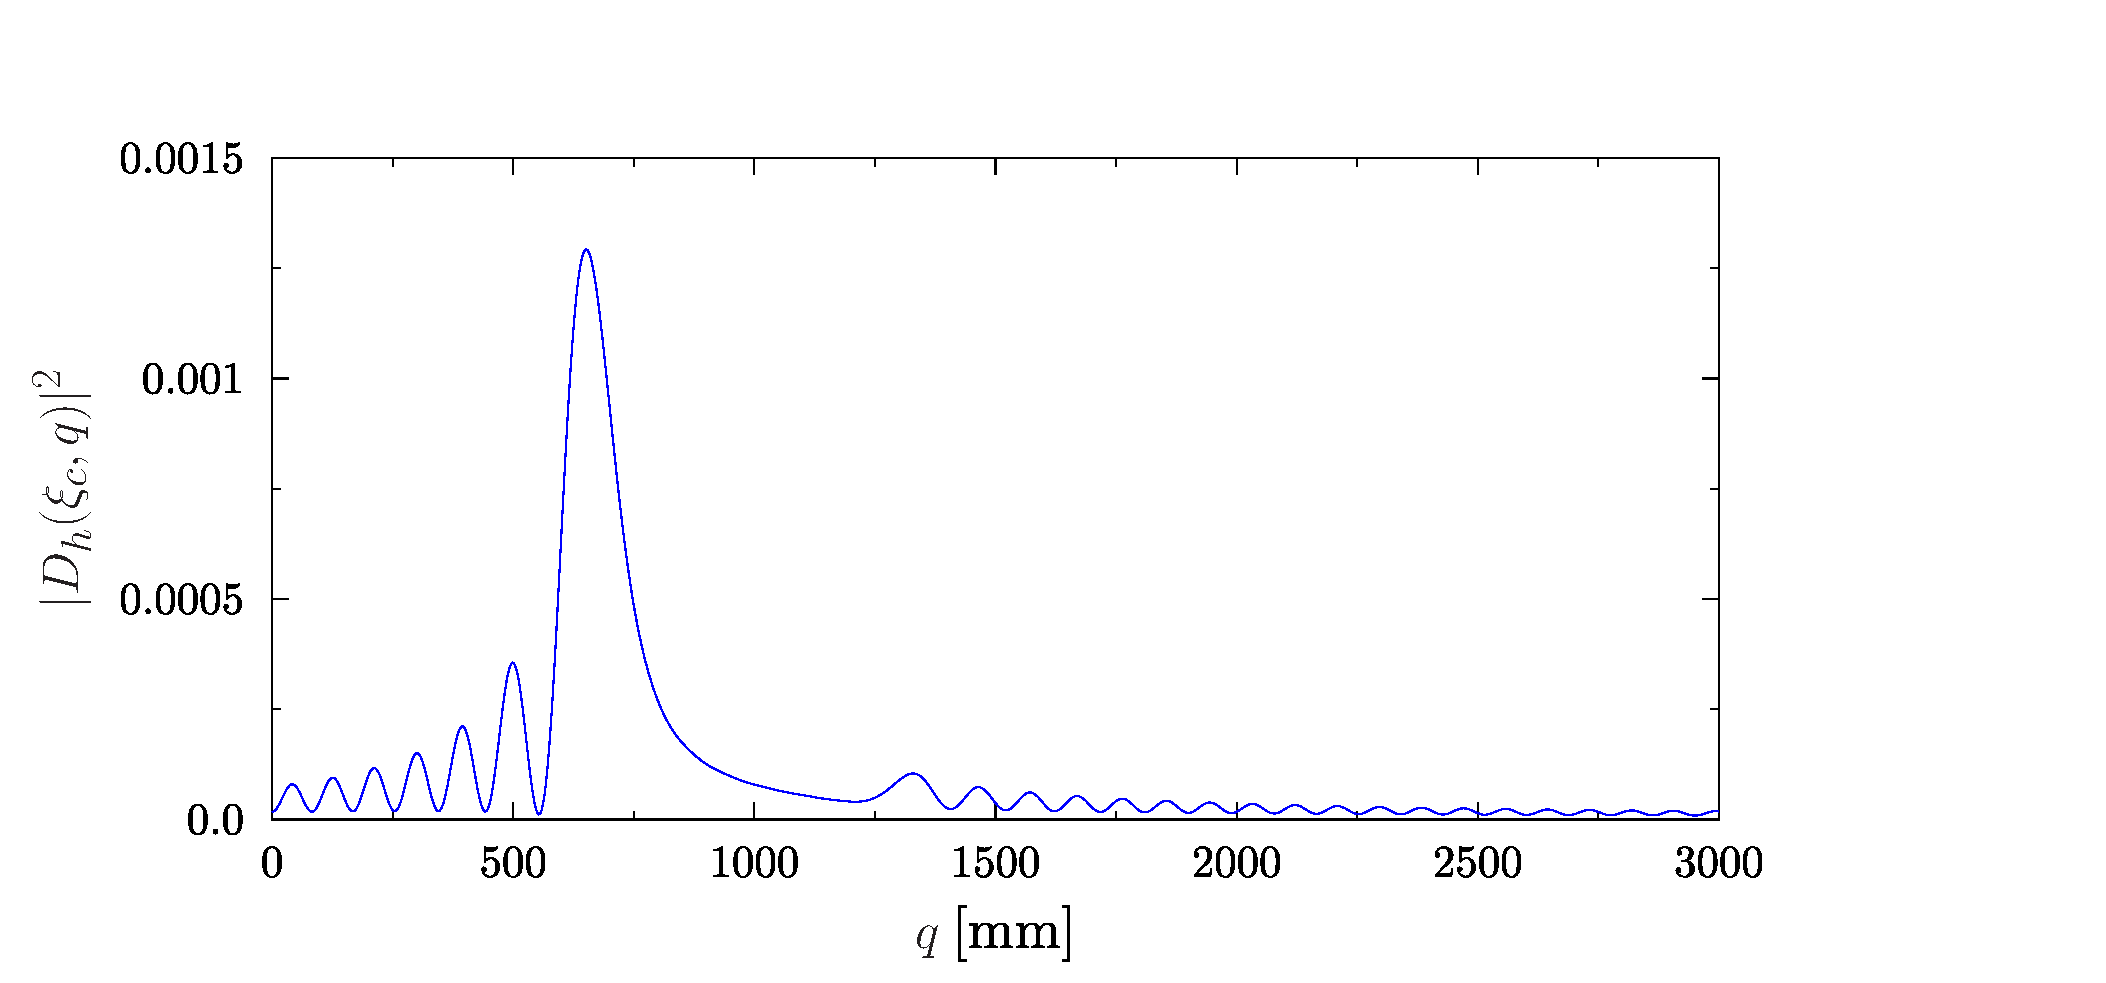
\includegraphics[width=0.96\textwidth]{bent1m8keV.eps}

\begin{picture}(0,0)
\setlength{\unitlength}{1cm}
\put(-1.5,3){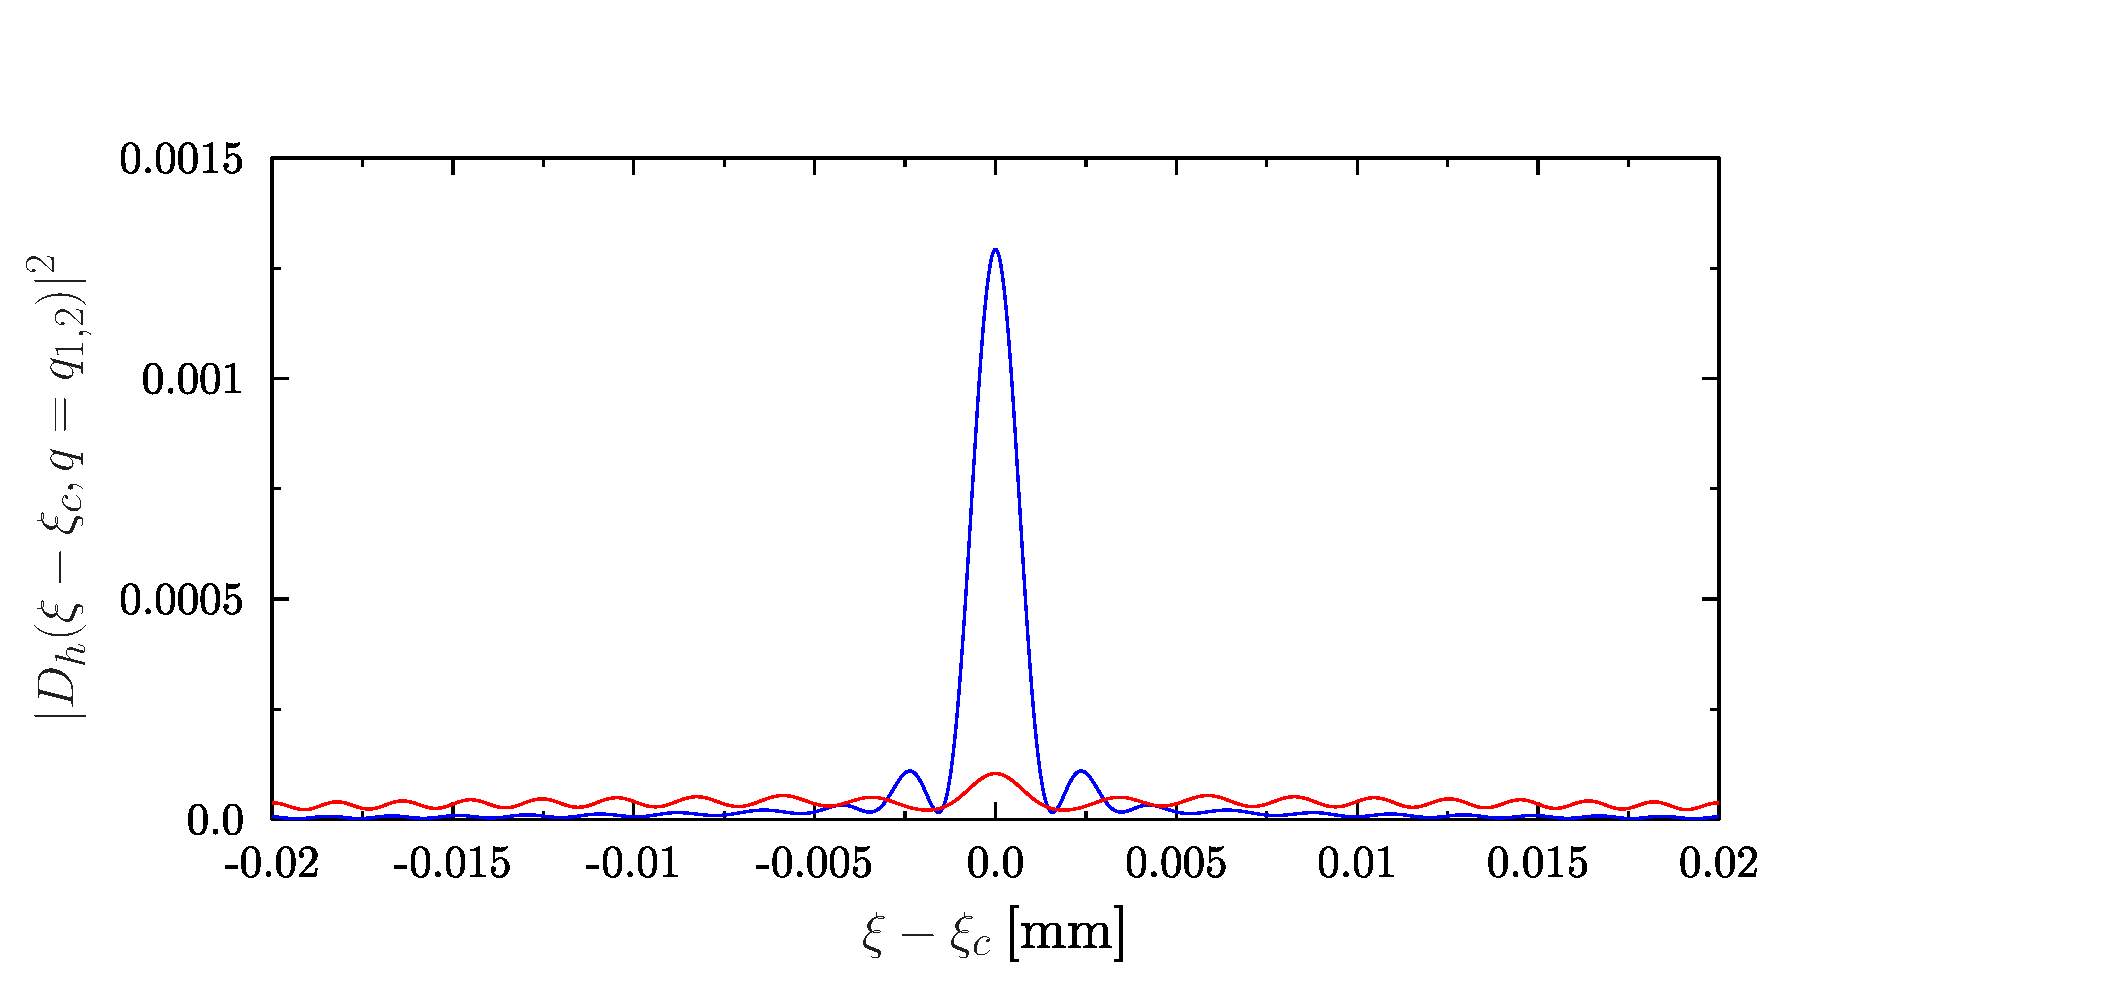
\includegraphics[width=0.46\textwidth]{bent1m8keV_profile.eps}}
\end{picture}

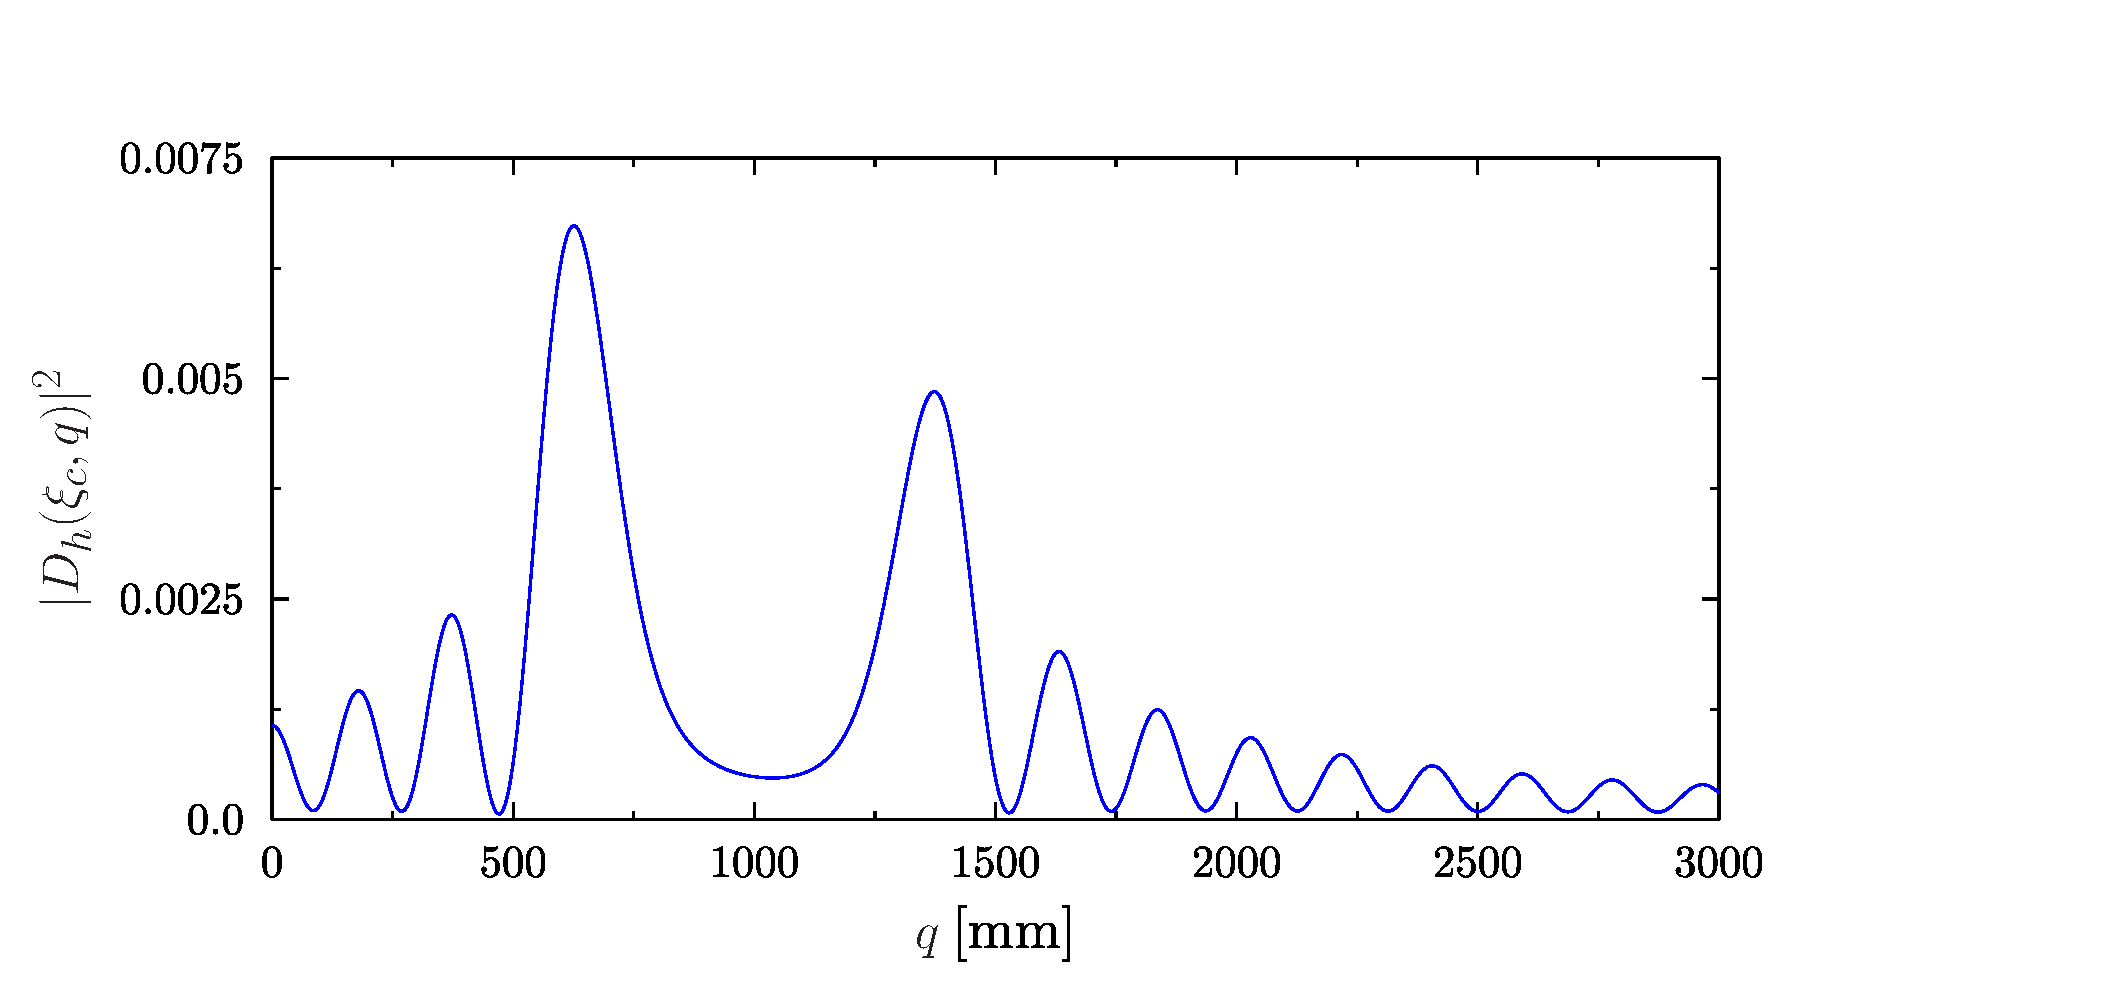
\includegraphics[width=0.96\textwidth]{bent1m17keV.eps}

\begin{picture}(0,0)
\setlength{\unitlength}{1cm}
\put(-1.1,3){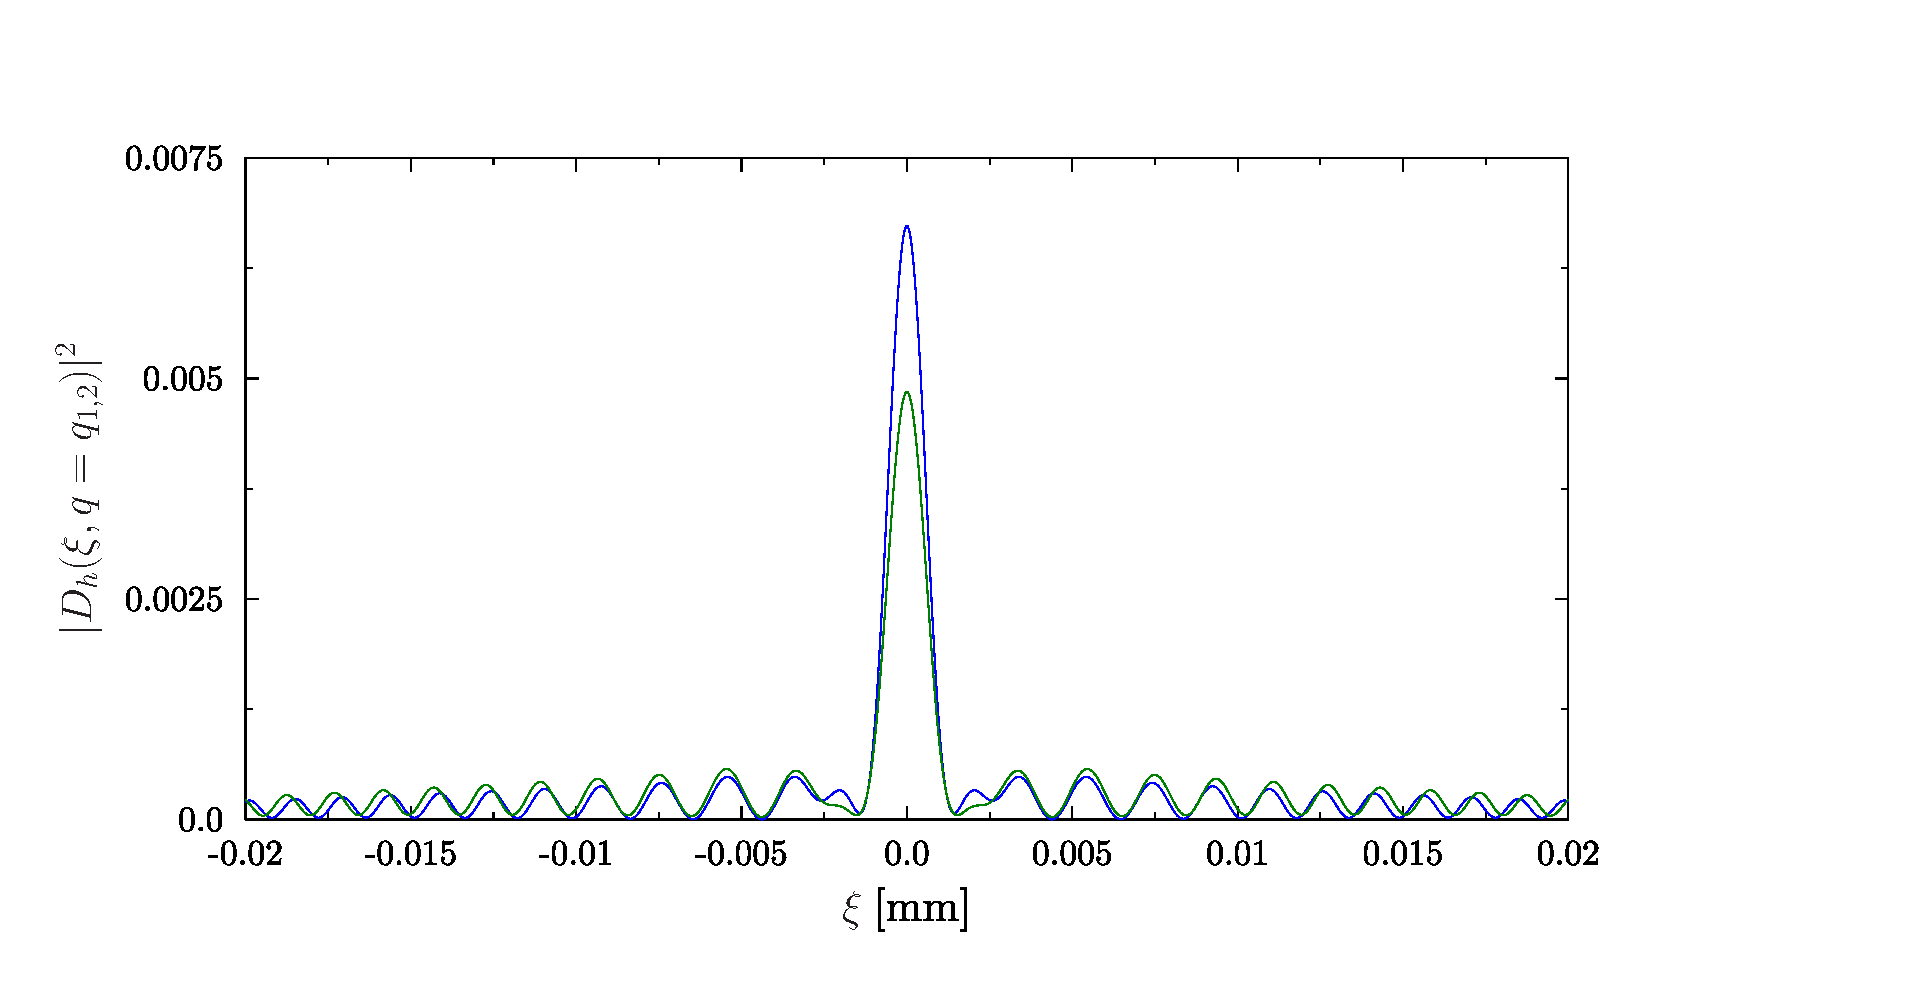
\includegraphics[width=0.46\textwidth]{bent1m17keV_profile.eps}}
\end{picture}

\end{figure}

It can be seen from equation~(\ref{eq:Dhpropagated}) that the intensity function $|D_h(s_0,s_h)|^2$ as a function of $\xi$ is symmetric around $\xi_c=-a q L_e / (2 q_e R \cos\theta_B)$. This denotes the lateral shift of the intensity profiles (the axial intensity profiles of Fig.\ref{fig:8keV}c and \ref{fig:8keV}d are actually calculated as a function of $(\xi-\xi_c)$. \todo{ Make a plot vs $\xi$ to see how it changes: IT CHANGES  $\approx -a/2$... TOO MUCH??}

\subsection{Semianalytical approach in asymmetric Laue geometry to obtain the CLE}
\label{sec:LaueCompatibilityCLE}

In this section we demonstrate, for the general case of asymmetric Laue, how the CLE can be obtained from the dynamical theory in the limit of zero thickness. To obtain this result we first summarize the results of \cite{GuigayFerrero2016} that give the expression of the diffracted field at the exit face of the crystal, which is then propagated to the image at a distance $q$. This expression has to be evaluated numerically (semi-analytically). It is shown that in the limit of zero thickness, this expression corresponds to a cylindrical wave focused in a position dictated by an expression that coincides with the CLE.

The same procedure used in section~\ref{sec:LaueNewCLE} is applied here, but it is more complicated for asymmetric reflection because of the larger number of parameters and the mathematical complexity of the Kummer function. The reflected amplitude versus the $\xi$ coordinate at negligible distance from the exit crystal surface is expressed by the following integral over the variable $\eta=\xi-\tau/\gamma$

\begin{equation}
\label{eq:unpropagatedkummer}
    D_h(\xi,0) = 
    \int_{-a}^{a} \gamma\frac{d\eta}{\sqrt{\lambda p}}
    e^{i k \gamma^2
    \frac{(\xi-\eta)^2}{2p}+i \phi(\xi,\eta)
    }
     M(\frac{i\Omega}{A},1,i g k \frac{a^2-\eta^2}{R}),
\end{equation}
where $\gamma=\cos\theta_1/\cos\theta_2$, $a=t \sin\theta_B/(2\cos\theta_1)$,


\begin{multline}
    \phi(\xi,\eta) =\frac{k}{2R}[-\mu_2\gamma^2(\xi-\eta)^2
    +a_2\gamma(\xi-\eta) \\
    -\mu_1(a+\xi)^2 
    +a_1(a+\xi)
    -2g(a+\xi)(\xi-\eta)],
\end{multline}
the parameters $\mu_{1,2}$, $a_{1,2}$ and $A$ \inred{and $g$} are given in the Appendix~\ref{appendix:Deformation},
\inred{$g=A\gamma R/ k \sin^22\theta_B$  \todo{$k$???}},
and $\rho=\nu/(1-\nu)$ with $\nu$ the Poisson ratio.   
The reflected amplitude $D_h(\xi,q)$ at distance $q$ downstream the crystal is again obtained using equation~(\ref{eq:Fresnel}), therefore by double integration over $\eta$ and $\xi'$. The $\xi'$-integration can be again performed analytically. The remaining $\eta$-integration involving the Kummer function is carried out numerically \cite{GuigayFerrero2016}. We consider this approach as semi-analytical, in contrast to the approach used by \cite{Nesterets} which is based on a numerical solution of the TTE.

We are now interested in the limit this \inred{semi-analytical} formulation in the case of vanishing crystal thickness ($a\rightarrow0{}$), for comparison with the CLE. In this limit, the Kummer function is equal to unity in equation~(\ref{eq:unpropagatedkummer}), and the integral can be replaced by $2a$ times the integrand evaluated at $\eta=a=0$, therefore
\begin{equation}
\label{eq:14reduced}
    D_h(\xi,0) = \frac{2 a \gamma}{\sqrt{\lambda p}} e^{\frac{i k \xi^2}{2}(\frac{\gamma^2}{p}-\frac{\mu_2\gamma^2+\mu_1+2g}{R})}.
\end{equation}

This is the expression of the amplitude of a cylindrical wave focused at the distance $q$ such that
\begin{equation}
    \frac{1}{q}+\frac{\gamma^2}{p}-\frac{\mu_2\gamma^2+\mu_1+2g}{R}=0. 
\end{equation}
Using the identity $\mu_1+\gamma^2\mu_2+2g=(\cos\theta_2-\cos\theta_1)/\cos^2\theta_2$, which is demonstrated in Appendix~\ref{appendix:Deformation}, the focusing condition is 
\begin{equation}
    \frac{1}{q}+\frac{\gamma^2}{p}+\frac{\cos\theta_1-\cos\theta_2}{R\cos^2\theta_2}=0,
\end{equation}
or,
\begin{equation}
    \frac{\cos^2\theta_2}{q}+\frac{\cos^2\theta_1}{p}+\frac{\cos\theta_1-\cos\theta_2}{R}=0,
\end{equation}
which is the CLE (equation~(\ref{eq:CLE})) for the Laue case, with the correspondence $p \rightarrow L_0$, $q \rightarrow -L_h$, $R \rightarrow -R$, $\theta_1 \rightarrow \varphi_0$ and $\theta_2 \rightarrow \varphi_h$


\section{Relevance of the lens equation in the symmetric Bragg case}
\label{sec:BraggGeometry}
Let us consider the case of a flat non-absorbing crystal plate (without bending), in symmetrical Bragg geometry. The fact that experimental results and also numerical calculations \cite{Honkanen2018} of Bragg diffraction with plane crystals do not show any focusing effect (contrary to Laue case), can be loosely explained by the following intuitive approach. Consider that any geometrical ray emitted from a real distant point-source produces a reflected ray at the point of incidence on the crystal surface, with a reflectivity coefficient equal to the complex reflectivity of the incident plane wave having the same glancing angle of incidence $\theta=\theta_B+\Delta\theta$ as the geometrical ray under consideration
\begin{equation}
\label{eq:braggDiffProfile}
    r(\Delta\theta) = \sqrt{1-\left(\frac{\Delta\theta\sin2\theta_B}{|\chi_h|}\right)^2} + i \frac{\Delta\theta\sin2\theta_B}{|\chi_h|} =
    e^{i \arcsin{\frac{\Delta\theta \sin2\theta_B}{ |\chi_h|}}}.
\end{equation}

Note that $|r(\Delta\theta)|^2$ is the usual diffraction profile. Taking the origin of coordinates at the point corresponding to $\theta=\theta_B$, the reflected wave-amplitude along an axis $O\xi$ situated in the diffraction plane and perpendicular to the reflected direction, at negligible distance from the crystal, may be approximated by setting  $\Delta\theta=\xi/p$ in equation~(\ref{eq:braggDiffProfile}):
\begin{equation}
    D(\xi) = e^{i \arcsin{\frac{\xi \sin2\theta}{p |\chi_h|}}}.
\end{equation}

No focusing effect is expected from this amplitude distribution, because the phase function $\arcsin(\xi \sin2\theta/ (p |\chi_h|))$, being an odd function of $\xi$, has no second-order term characteristic of a focusing effect; the first-order term produces a lateral shift of the image. There is no equivalent to the dynamical focusing length $q_{dyn}$ introduced in the Laue case. The reflected beam is indeed divergent, as in the case of a usual mirror.

The focusing properties of cylindrically bent crystals in symmetric Bragg geometry were simulated by \inblue{\cite{sutter2010}, using a finite-defference method, and by \cite{honkanen2017, Honkanen2018}}, using a finite-element method for numerical solution of the TTE. The obtained phase distribution of the reflected wavefront shows a parabolic shape, with concavity inversion as compared to the parabolic phase distribution of the incident wavefront. This is a clear indication of a single real focusing effect, which is indeed confirmed by simulating the reflected wave propagation. The obtained focusing distances are indeed in good agreement with the CLE which is $L_0^{-1}+L_h^{-1}=2/(R\inred{_c} \sin\theta_B)$ in this case.
These results can be interpreted as follows: because of the deformation phase factor $\exp(-i\vec h. u(\vec x_s))$, the reflected waves acquire a quadratic phase distribution with the sign corresponding to a cylindrically convergent wave.



\section{Polychromatic geometric focusing}
\label{sec:polychromatic}

As pointed out by \cite{CK}, the monochromatic focusing effect \todo{monochromatic focusing?} must not be confused with the polychromatic focusing effect \cite{handbook} \todo{add Schulze et al. 1998, Martison et al. 2015} obtained by varying the wavelength of the reflected rays in order to satisfy the exact Bragg condition on the crystal surface (the position of the point $O$ and the change of the Bragg angle along the crystal surface. The asymmetry angle $\alpha$ is constant. The equation $\varphi_0+\varphi_h=2\alpha$ in Laue case ($\varphi_0+\varphi_h=2\alpha+\pi$ in Bragg case) implies $\Delta\varphi_0+\Delta\varphi_h=0$. Using equations~(\ref{eq:angles}) and  (\ref{eq:angles2}) we obtain the polychromatic crystal lens equation
\begin{equation}
\label{eq:polychromaticfocusing}
\frac{{\cos {\varphi _o}}}{{{L_0}}} + \frac{{\left| {\cos {\varphi _h}} \right|}}{{{L_h}}} = \frac{2}{R_c},
\end{equation}
or, in the notation of section~\ref{sec:dynamlicalLaue}, $-\cos\theta_1/p + |\cos\theta_2|/q=2/R$. Equation~(\ref{eq:polychromaticfocusing}) is usually referred as "geometric focusing" condition \todo{REF?}. \inblue{This polychromatic focusing effect was also discussed for flat Laue crystals \cite{sanchezdelrio1994}.} Equation~(\ref{eq:polychromaticfocusing}) is applied for focusing a polychromatic beam by a thin crystal \inred{instead of the CLE} . Another equation has been introduced in order to deal with the effects of a finite crystal thickness \cite{PengQi}\footnote{\cite{PengQi} found another polychromatic condition in Laue geometry. A ``single-ray focusing" condition is obtained by considering different wavelengths in an individual geometrical incident ray. Each wavelength fulfils the Bragg law in a given point along the ray path along traversing the crystal. This give rise to different reflected rays which propagate with different directions and may come together in a "single-ray focal point". This effect is not considered here, and we restrict our discussion to thin bent crystals. }.


It is easy to see that equations (\ref{eq:CLE}) (for monochromatic wavefronts) and (\ref{eq:polychromaticfocusing}) (for polychromatic beams) coincide in the symmetric Bragg case (for which $\cos\varphi_o=-\cos\varphi_h=\sin\theta_B$), but not necessarily for the \inred{\sout{generic}} symmetric Laue case. In the symmetric Laue case, for which $\cos\varphi_o=\cos\varphi_h=\cos\theta_B$, the monochromatic condition (equation~\ref{eq:CLE}) is reduced to $L_0=L_h$ and the polychromatic condition (equation~\ref{eq:polychromaticfocusing}) is then $L_0=L_h=R_c\cos\theta_B$, which corresponds to Rowland geometry. Therefore the equations of monochromatic (\ref{eq:CLE}) and polychromatic (\ref{eq:polychromaticfocusing}) focusing coincide for symmetric Laue case only if the Rowland condition is satisfied.\footnote{\cite{CK} stated that they coincide if a symmetrical reflection is used {\it or} the Rowland condition is fulfilled, which is false in the symmetric Laue off-Rowland}

The equations for monochromatic focusing and polychromatic focusing do coincide, \inred{in all cases,} if the Rowland condition $L_0=R_c\cos\varphi_0$ is satisfied, since they both give the same $L_h=R_c|\cos\varphi_h|$. The bent crystal is then reflecting only a narrow energy band, because the angle of incidence on the local reflecting planes does not change along the bent crystal surface.
In synchrotron dispersive EXAFS beamlines, the objective is to reflect a large energy bandwidth (polychromator), therefore they work off-Rowland condition with a large source-to-crystal distance. The use of symmetric Bragg reflection in most polychromators guarantees that the polychromator focuses a broad-bandwidth (up to ~1 keV) beam onto a small spot \cite{Tolentino:ms0206}. The focal distance would be $L_h=R_c\cos\theta_B/2$.

Laue polychromators are also used in synchrotron beamlines \todo{REF}.
\inred{As discussed before,
polychromatic CLE (equation (\ref{eq:polychromaticfocusing})) and monochromatic CLE (equation (\ref{eq:CLE})) coincide only in Rowland configuration. Therefore it would be impossible to work off-Rowland  (a necessary condition to obtain a large energy bandwidth in dispersive EXAFS). However, as stated in section~\ref{sec:dynamlicalLaue} the use of the monochromatic CLE (equation (\ref{eq:CLE})) is not adequate in Laue, and should be replaced by a generalized CLE (equation~(\ref{eq:newCLE})) which includes postulates of the dynamical theory.}
Equation ~(\ref{eq:newCLE}), valid for a crystal of any thickness in symmetric Laue geometry, gives $L_h \approx R_c \cos\theta_B + (R_c \cos\theta_B) ^2 / q_{dyn}$ in the case of a very large source-to-crystal distance. The coincidence of polychromatic and monochromatic focusing conditions is then realised if
$R_c \cos\theta_B /2 = R_c \cos\theta+ (R_c \cos\theta_B) ^2 / q_{dyn}$ which implies $R_c=-q_{dyn}/2$.
This means a real focus at the focal distance $|L_h|=q_{dyn}/4$ \todo{WHY? I get /2} with beam incident in the convex side ($R_c<0$). The Laue crystal can then be optimized to verify this condition by choosing the right $q_{dyn}$. This is done by selecting an adequate crystal thickness to obtain the required $q_{dyn}$ value \cite{Mocella2004} \cite{Mocella2008}. 


\section{Summary and conclusions}
\label{sec:summary}
A crystal lens equation (CLE) based on the conservation of the parallel component of the wavevector in the diffraction process is obtained (equation~\ref{eq:CLE}). It includes all cases of symmetric and asymmetric Laue and Bragg geometries. It differs from the previous formulation \cite{CK} in the Laue case. However, the lens equation is actually of little practical interest in the Laue case, because it can be applied only if the crystal is very thin, and it neglects important effects resulting from the dynamical theory of diffraction, like the focusing of the Borrmann triangle. We derived a modified lens equation (\ref{eq:newCLE}) in the case of symmetric geometry which overcomes this restriction. Consistently, it converges to the CLE in the case of a crystal with zero thickness, a case that has little utility. The generic case of arbitrary asymmetry is left for a future investigation.

The application of the CLE (equation~\ref{eq:CLE}) is restricted to monochromatic focusing. Polychromatic focusing, as used in the polychromators of dispersive EXAFS beamlines, happens when the wavelength of the reflected rays changes to exactly match the Bragg angle. This condition is given by a different lens equation (\ref{eq:polychromaticfocusing}). This implies a specular reflection of the rays on the Bragg planes that is, in general, incompatible with the CLE or the results of dynamical theory, except for the Bragg symmetric case, or for rays matching exactly the Bragg condition thus verifying Laue equation. Therefore, polychromatic and monochromatic focusing must be treated separately. It has been demonstrated that focii predicted by monochromatic and polychromatic focusing conditions coincide if the source is situated on the Rowland circle. Moreover, such coincidence is also true for any source position (off-Rowland) in symmetric Bragg geometry, but not in symmetric Laue geometry. Here, for the Laue symmetric case, both polychromatic and monochromatic focii can match if the modified lens equation~(\ref{eq:newCLE}) is used instead, but requires a particular choice of the crystal thickness.

% The case of symmetric Bragg geometry seems to be of particular practical interest, because of simultaneous polychromatic and monochromatic focusing. Moreover, the CLE can then be used to predict the focus position with good accuracy. Therefore, the CLE appears to be more relevant in the Bragg case rather than in the Laue case.


% \ack{Acknowledgements}
% A large part of this work comes from ...


\bibliography{iucr} % reads iucr.bib with items
\bibliographystyle{iucr}
%\referencelist{library}

\appendix
\section{The Crystal Lens Equation deduced from the phase-factor of the Takagi-Taupin equations}
\label{appendix:CLE}.

In a crystal under a deformation field $\vec u(\vec r)$, the polarizability of a crystal can be taken as $\chi(\vec r-\vec u(\vec r))$, where $\chi(\vec r)$ is the polarizability of the non-deformed crystal. The Fourier components of the electric susceptibility $\chi_h$ and $\chi_{\bar h}$ are multiplied by the phase factors $\exp(-i k \vec h . \vec u (\vec r))$ and $\exp(+i k \vec h . \vec u (\vec r))$, respectively, in the Takagi-Taupin equations which describe  the propagation inside the deformed crystal.

In the case of a very thin crystal, multiple scattering can be neglected. The incident ray at the point of coordinate x on the crystal surface is simply afected by a phase factor 
\begin{equation}
    e^{-i k \vec h . \vec u(x)} = e^{i k (\cos\varphi_h-\cos\varphi_0) \frac{x^2}{2 R_c} },
\end{equation}
which is easily obtained by using $\vec u(x) = -(x^2/(2R))\vec n$ and $\vec n . \vec h = \vec n.(\vec k_h - \vec k_0) = k(\cos\varphi_h-\cos\varphi_0)$. 

The incident cylindrical wave $\phi_0(\tau)=\exp[i k \tau^2 / (2L_0)]$, where $\tau$ is the coordinate along the axis $O\tau$ perpendicular to the direction $Os_0$ of Bragg incidence (see Fig.~\ref{fig:vectors}), produces the following phase distribution along the axis $O\xi$ perpendicular to the direction $Os_h$ of Bragg reflection 
\begin{equation}
    D_{inc}(\xi) = e^{i k \frac{\xi^2}{2L_0}\left(\frac{\cos\varphi_0}{\cos\varphi_h}\right)^2},
\end{equation}
where we use the geometric relations $x=\tau/cos\varphi_0=\xi/|\cos\varphi_h|$. The amplitude of the Bragg-reflected wave along the axis $O\xi$ is
\begin{equation}
\label{eq:A4}
    D_h(\xi) = e^{i k
    \frac{\xi^2}{\cos^2\varphi_h}\left(\frac{\cos\varphi_h-\cos\varphi_0}{2R_c} + \frac{\cos^2\varphi_0}{2L_0}\right)},
\end{equation}
corresponding (in Laue or Bragg geometry), to a real or virtual focus if the phase of this function is negative or positive respectively. Using the notations defined in section~\ref{sec:CLE}, a real focus corresponds to $L_h<0$ in Laue case and to $L_h>0$ in Bragg case; similarly, a \inred{virtual} focus corresponds to $L_h>0$ in Laue case and to $L_h<0$ in Bragg case. This means that \inred{a cylindrical wave collapsing to the focus has the form} $D_h(\xi) = \exp(\pm i k \xi^2 / (2L_h))$ \inred{with positive phase sign} in Laue \inred{and negative phase sign} in Bragg. This expression can be rewritten \inred{for both Bragg and Laue cases} as
\begin{equation}
\label{eq:A5}
D_u(\xi) = e^{i k \frac{\xi^2}{2 L_h}\frac{|\cos\varphi_h|}{\cos\varphi_h}}.   
\end{equation}
Comparing equations~(\ref{eq:A4}) and (\ref{eq:A5}), we finally obtain
\begin{equation}
    \frac{\cos\varphi_h-\cos\varphi_0}{R_c}+
    \frac{\cos^2\varphi_0}{L_0}=\frac{|\cos\phi_h|\cos\varphi_h}{L_h},
\end{equation}
which is equivalent to the lens equation (\ref{eq:CLE}).

\section{Derivation of the influence functions from the integral form of the Takagi-Taupin equations}
\label{appendix:TTEintegral}

\inblue{


The IF for a point-source of oblique coordinates $(\sigma_0,\sigma_h)$ is related to the incident wave $\exp(i\vec k_0 . \vec x) \delta(s_h-\sigma_h)$, corresponding to $D_{inc}=\delta(s_h-\sigma_h)$. The refracted amplitude in the crystal is $D_{ref}(\sigma'_0,\sigma'_h)=\exp(i k \chi_0 s'_0/2)\delta(s'_h)$ by using the variables $s'_{0,h}=s_{0,h}-\sigma_{0,h}$.
According to equation~(\ref{eq:functionsG}b), the refracted amplitude takes the form
\begin{equation}
    G_{ref}=\exp[-i\frac{k}{2}\chi_0(s_0+s_h)+i \phi_2(s_h)] D_{ref}(s'_0,s'_h) = E\delta(s'_h)
\end{equation}
where $E=\exp[-i (k/2) \chi_0 (s_0 + s_h) + i \phi_2(\sigma_h)]$ is a constant phase term. Considering the $G(s_o,s_h)$  as functions $G_h(s'_0,s'_h)$ of $s'_0$ and $s'_h$, the TTE (\ref{eq:TTEsimple}) are expressed as

\begin{subequations}
\label{eq:TTEappendix}
\begin{align}
    \frac{\partial G_0(s'_0,s'_h)}{\partial s'_0}=&i\frac{k}{2}\chi_{\bar h} G_h(s'_0,s'_h) \\
    \frac{\partial G_h(s'_0,s'_h)}{\partial s'_h}=&i\frac{k}{2}\chi_{h} G_0(s'_0,s'_h) -i A (s'_0+\sigma_0)G(s'_0,s'_h).
\end{align}
\end{subequations}

It is then convenient to rewrite them in terms of the functions $F_{0,h}(s'_0,s'_h)$ such that
\begin{subequations}
\label{eq:TTEappendix2}
\begin{align}
    G_0(s'_0,s'_h) =& e^{-iA\sigma_0s'_h} F_0(s'_0,s'_h),\\
    G_h(s'_0,s'_h)=&i\frac{k}{2}\chi_{h} e^{-iA\sigma_0s'_h} F_h(s'_0,s'_h).
\end{align}
\end{subequations}

Consequently, equations (\ref{eq:TTEappendix2}) are rewritten as
\begin{subequations}
\label{eq:TTEappendix3}
\begin{align}
    \frac{\partial F_0}{\partial s'_0}=&-\Omega F_h \\
    \frac{\partial F_h}{\partial s'_h}=&F_0-i A s'_0 F_h,
\end{align}
\end{subequations}
where $\Omega=k^2\chi_h\chi_{\bar h}/4$. The refracted amplitude is $F_{ref}=E\delta(s'_h)$. Equations (\ref{eq:TTEappendix3}) can be put in the form of integral equations:
\begin{subequations}
\label{eq:TTEappendixIntegral}
\begin{align}
    F_0(s'_0,s'_h) =& E \delta(s'_h) -\Omega\int_0^{s'_0} d\xi_0F_h(\xi_0,s'_h),\\
    F_h(s'_0,s'_h)=& \int_0^{s'_h} d\xi_h F_0(s'_0,\xi_h) - i A s'_0 \int_0^{s'_h} d\xi_h F_h(s'_0,\xi_h).
\end{align}
\end{subequations}

The following solution is based on the process of multiple Bragg scattering. Starting from 
$(F_0,F_h)=(E\delta(s'_h),0)$, we obtain the first-order term, or kinematical expression, $(F_0,F_h)=(E\delta(s'_h), E)$. Successive terms are obtained by iteration. The transmitted and reflected amplitudes are made up by terms of  even and odd order, respectively. Alternatively, we can combine equations \inred{(\ref{eq:TTEappendixIntegral})} into a single integral equation for the reflected amplitude
\begin{equation}
    \label{eq:TTEappendixSingleIntegral}
    F_h(s'_0,s'_h) = E - \Omega \int_0^{s'_h} d \xi \int_0^{s'_0}d \xi F_h(\xi_0,\xi_h) - i A s'_0 \int_0^{s'_h} d\xi_h F_h(s'_0,\xi_h).
\end{equation}
By iteration starting from $F_h=\exp(i\Gamma)$, we obtain

\begin{align}
    \label{eq:TTEappendixSeries}
    F_h(s'_0,s'_h) = E [ 1 - 
    (\Omega+i A) s'_0s'_h + ...+
    \nonumber \\
    (\Omega+iA)(\Omega+2iA)...(\Omega+niA)
    \frac{(-s'_0 s'_h)^n}{n!n!}
    +...]
\end{align}

The above bracketted series can be expressed as:
\begin{align}
    \label{eq:Series}
    \sum_{n=0}^{\infty} (1-i\frac{\Omega}{A})
    (2-i\frac{\Omega}{A})...
    (n-i\frac{\Omega}{A})
    \frac{(i-A s'_0 s'_h)^n}{n!n!}=&\\
    M(1-iA\frac{\Omega}{A},1,-iAs'_0 s'_h) = & \\
    e^{-iAs'_0 s'_h}M(i\frac{\Omega}{A},1,iAs'_0s'_h),
\end{align}
where we used the definition (equation~(\ref{eq:kummerSeries})) of the Kummer function and its known property $M(a,b,z)=\exp(z)M(b-a,b,-z)$.
The corresponding expression for $F_0(s'_0,s'_h)$ is then easily obtained by using formula \inred{(\ref{eq:TTEappendix3}b)}.

Taking into account  formulas \inred{(9)}, we obtain
\begin{align}
\label{eq:appendixFinal}
  &D_h= \nonumber \\
  &i\frac{k}{2}\chi_h E
  e^{i(\frac{k}{2}\chi_0(s_0+s_h)-
  \phi_1(s_0) + A s_0 s_h -A \sigma_0 s'_h - As'_0 s'_h)}
  M(i\frac{\Omega}{A},1,iA,s'_0 s'_h)
  = \nonumber \\
  &i\frac{k}{2}\chi_h 
  e^{i(\frac{k}{2}\chi_0(s'_0+s'_h)+
  \phi_2(s_h) - \phi_1(s_0) + A s_0 s_h )}
  M(i\frac{\Omega}{A},1,iA,s'_0 s'_h)
  = \nonumber \\
  &i\frac{k}{2}\chi_h 
  e^{i\frac{k}{2}\chi_0(s'_0+s'_h)
  -i \vec h . \vec u(s_0,\sigma_h)}
  M(i\frac{\Omega}{A},1,iA,s'_0 s'_h)
\end{align}

in which we use  the relation $s_0s_h-\sigma_0 s'_h - s'_0 s'_h=s_0 s_h - s_0 s'_h = s_0 \sigma_h$.
}

% An incident monochromatic wave of any form, can also be expressed as a modulated plane wave $D_{inc}(\vec x)\exp(i\vec k_0. \vec x)$ defining a continuous distribution of coherent point-sources on the crystal surface, according to the general Huyghens principle in optics. The influence functions, or propagators, are the solutions of the TTE corresponding to these point-sources. The IF for a point-source of coordinates $(\sigma_0,\sigma_h)$, in the case of crystals with deformation that verify equation~(\ref{eq:cylinder}), are derived in \cite{GuigayFerrero2016} by formulating the TTE as integral equations and solving them by iteration, starting from the undiffracted term $D_{inc}(s_0,s_h\inred{;\sigma_0,\sigma_h})=\exp[ik(s_0-\sigma_0)]\delta(s_h-\sigma_h)$, with $\delta$ the Dirac delta. The result for the diffracted field $D_h$ is
% \begin{multline}
% \label{eq:preKummer}
%     D_h(s_0,s_h) =  \frac{i k}{2} \chi_h e^{(ik/2) \chi_0 (s'_0 + s'_h)} e^{i A s'_o s'_h - i\vec h.\vec u(s_o,\sigma_h)} \times
%     \\
%     [1 + \sum_{i=1}^\infty \frac{(\Omega + i A )(\Omega+2iA)...(\Omega+niA)}{n!n!}(-s'_0s'_h)^n],
% \end{multline}
% where $s'_{0,h}=s_{0,h}-\sigma_{0,h}$ and $\Omega = k^2 \chi_h \chi_{\bar h}/4$. The first exponential stands for the effects of refraction and normal absorption. For $A\ne0$, the equation~(\ref{eq:preKummer}) can be expressed as
  


\section{General expression of the phase factor and derivation of equation~(\ref{eq:14reduced})}
\label{appendix:Deformation}.

The components of the displacement field, in the case of meridional bending of radius $R$ are \cite{Nesterets}:
\begin{equation}
    u_x = -\frac{x(z-t/2)}{R}; \, u_z=\frac{x^2+\rho(z-t/2)^2}{2R},
\end{equation}
with $\rho=\nu/(1-\nu)$, and $\nu$ the Poisson ratio (we used $\nu$~= 0.22 for Silicon in the calculations in this paper). 
Note that $h_x=k(\sin\theta_2-\sin\theta_1)$, $h_z=k(\cos\theta_2-\cos\theta_1)$.
In terms of the oblique coordinates $(s_0,s_h)$ along $\vec k_{0,h}$, such that $z=s_0\cos\theta_1 + s_h \cos\theta_2$ and $x=s_0 \sin\theta_1+s_h\sin\theta_2$ , 
it is found, by lengthy but simple calculations and with omission of a constant term, that $\vec h.\vec u=-A s_0 s_h + \phi_1(s_0) -\phi_2(s_h)$,  
with the following definitions
\begin{equation}
    A = -(2 k \sin\theta_B /R)\sin\alpha[1+(1+\rho)\cos\theta_1\cos\theta_2]
\end{equation}
\begin{align}
    \phi_1(s_0) &= \frac{k}{2R}[\mu_1(s_o\sin2\theta_B)^2-a_1 s_0\sin2\theta_B] \nonumber \\
    \phi_2(s_h) &= -\frac{k}{2R}[\mu_2(s_h\sin2\theta_B)^2-a_2 s_h\sin2\theta_B],
\end{align}
where $\gamma=\cos\theta_1/\cos\theta_2$, $\theta_{1,2}=\alpha\pm \theta_B$,
% $a_{\inred{1,2}}=t \sin2\theta_B / (2\cos\theta_{1\inred{,2}})$,
\begin{align}
   g &= -\sin\alpha\frac{\gamma +(1+\rho)\cos^2\theta_1}{(\sin2\theta_B\cos\theta_B)}, \nonumber \\
   \mu_{1,2} &=\frac{\sin\alpha(\sin^2\theta_{1,2}+\rho\cos^2\theta_{1,2})+\cos\alpha\sin2\theta_{1,2}}{\sin2\theta_B\cos\theta_B}, \nonumber \\
   a_{1,2} &=t\frac{\cos\alpha\sin\theta_{1,2}+\rho\sin\alpha\cos\theta_{1,2}}{\cos\theta_B}. \nonumber
\end{align}

These formulas are simplified for a symmetric reflection ($\alpha=0$):
$A=0$, $\cos\theta_{1,2}=\cos\theta_B$, $\mu_{1,2}=\pm1/\cos\theta_B$, $a_{1,2}=\pm t\tan\theta_B$, $\phi_1$ and  $\phi_2$ have the same form $\phi(s)=[(s\sin2\theta_B)^2-s t \sin2\theta_B\sin\theta_B] / (2 R \cos\theta_B)$. 

The parameter $\rho$ is eliminated in the following expressions 
\begin{align}
    \mu_1+g=&\frac{\cos\alpha\sin2\theta_1-\sin\alpha(\gamma+\cos2\theta_1)}{\sin2\theta_B\cos\theta_B},
    \\
    \gamma^2\mu_2+g=&\frac{\gamma^2\cos\alpha\sin2\theta_2-\sin\alpha(\gamma+\gamma^2\cos2\theta_2)}{\sin2\theta_B\cos\theta_B}.
\end{align}

Using
\begin{align}
    &\sin2\theta_1+\gamma^2\sin2\theta_2 = \nonumber \\
    &2(\gamma\sin\theta_1\cos\theta_2+\sin\theta_2\cos\theta_1) =2\gamma\sin2\alpha,
\end{align}
and
\begin{align}
    &\cos2\theta_1+\gamma^2\cos2\theta_2=\nonumber \\
    &2\cos^2\theta_1-1+\gamma^2(2\cos^2\theta_2-1)=
    4\cos^2\theta_1-1-\gamma^2; \nonumber \\
    &\cos\alpha \sin2\alpha-\sin\alpha=\sin\alpha(2\cos^2\alpha-1)=\sin\alpha\cos\2\alpha. \nonumber
\end{align}
we obtain
\begin{align}
    \mu_1+\gamma^2\mu_2+2g =& \nonumber \\
    \sin\alpha
    \frac{2\gamma\cos2\alpha-4\cos^2\theta_1+1+\gamma^2}{\sin2\theta_B\cos\theta_B}, \nonumber 
\end{align}  
    
    
Furthermore, 
\begin{align}
    &\cos2\alpha+\cos2\theta_B = 
    2\cos\theta_1\cos\theta_2, \nonumber \\
    & \cos^2\theta_1+\cos^2\theta_2 = \nonumber \\
    & \frac{1+\cos(2\alpha+2\theta_B)}{2} + 
    \frac{1+\cos(2\alpha-2\theta_B)}{2} = \nonumber \\
    & 1+\cos2\alpha\cos2\theta_B, \nonumber \\
    &\frac{\mu_1+\gamma^2\mu_2+2g}{\sin\alpha} = \nonumber \\
    & \frac{2\cos\theta_1\cos\theta_2(\cos2\alpha-2\cos\theta_1\cos\theta_2)+\cos^2\theta_2+\cos^2\theta_1}{\cos\theta_B\sin2\theta_B\cos^2\theta_2} = \nonumber \\
    & \frac{\sin2\theta_B}{\cos\theta_B\cos^2\theta_2}. \nonumber 
\end{align}

Therefore:
\begin{align}
    \mu_1+\gamma^2\mu_2+2g = & \nonumber \\
    \frac{2\sin\alpha\sin\theta_B}{\cos^2\theta_B} = &
    \frac{\cos(\alpha-\theta_B)-\cos(\alpha+\theta_B)}{\cos^2\theta_2}=
    \frac{\cos\theta_2-\cos\theta_1}{\cos^2\theta_2}
\end{align}





     %-------------------------------------------------------------------------
     % The back matter of the paper - acknowledgements and references
     %-------------------------------------------------------------------------

     % Acknowledgements come after the appendices



     % References are at the end of the document, between \begin{references}
     % and \end{references} tags. Each reference is in a \reference entry.

%\begin{references}
%\reference{Author, A. \& Author, B. (1984). \emph{Journal} \textbf{Vol}, first page--last page.}
%\end{references}
%\cite{knuth84}

%\begin{thebibliography}{30}
%\expandafter\ifx\csname natexlab\endcsname\relax\def\natexlab#1{#1}\fi
%\expandafter\ifx\csname bibnamefont\endcsname\relax
%  \def\bibnamefont#1{#1}\fi
%\expandafter\ifx\csname bibfnamefont\endcsname\relax
%  \def\bibfnamefont#1{#1}\fi
%\expandafter\ifx\csname citenamefont\endcsname\relax
%  \def\citenamefont#1{#1}\fi
%\expandafter\ifx\csname url\endcsname\relax
%  \def\url#1{\texttt{#1}}\fi
%\expandafter\ifx\csname urlprefix\endcsname\relax\def\urlprefix{URL }\fi
%\providecommand{\bibinfo}[2]{#2}
%\providecommand{\eprint}[2][]{\url{#2}}
%
%\bibitem[{\citenamefont{Shvyd'ko}(2016)}]{GuigayFerrero2013}
%\bibinfo{author}{\bibfnamefont{Yu.}~\bibnamefont{Shvyd'ko}},
%\bibinfo{journal}{Phys. Rev. Lett.} \textbf{\bibinfo{volume}{116}},
%\bibinfo{pages}{080801} (\bibinfo{year}{2016}).
%
%%\bibitem[{\citenamefont{Guigay and Ferrero}]{ddd}
%%\bibinfo{author}{\bibfnamefont{Jean-Pierre}~\bibnamefont{Guigay}},
%%\bibinfo{author}{\bibfnamefont{Claudio}~\bibnamefont{Ferrero}},
% % \bibinfo{journal}{xxxx} \textbf{\bibinfo{volume}{xx}},
% % \bibinfo{pages}{xx} (\bibinfo{year}{2012}).
%
%\end{thebibliography}

%% Note added by Overleaf: If using bibtex, remove the "references" environment above, and uncomment the following lines.

%\bibliographystyle{iucr}
%\referencelist{iucr}

%      %-------------------------------------------------------------------------
%      % TABLES AND FIGURES SHOULD BE INSERTED AFTER THE MAIN BODY OF THE TEXT
%      %-------------------------------------------------------------------------
% 
%      % Simple tables should use the tabular environment according to this
%      % model
% 
% \begin{table}
% \caption{Caption to table}
% \begin{tabular}{llcr}      % Alignment for each cell: l=left, c=center, r=right
%  HEADING    & FOR        & EACH       & COLUMN     \\
% \hline
%  entry      & entry      & entry      & entry      \\
%  entry      & entry      & entry      & entry      \\
%  entry      & entry      & entry      & entry      \\
% \end{tabular}
% \end{table}
% 
%      % Postscript figures can be included with multiple figure blocks
% 
% \begin{figure}
% \caption{Caption describing figure.}
% 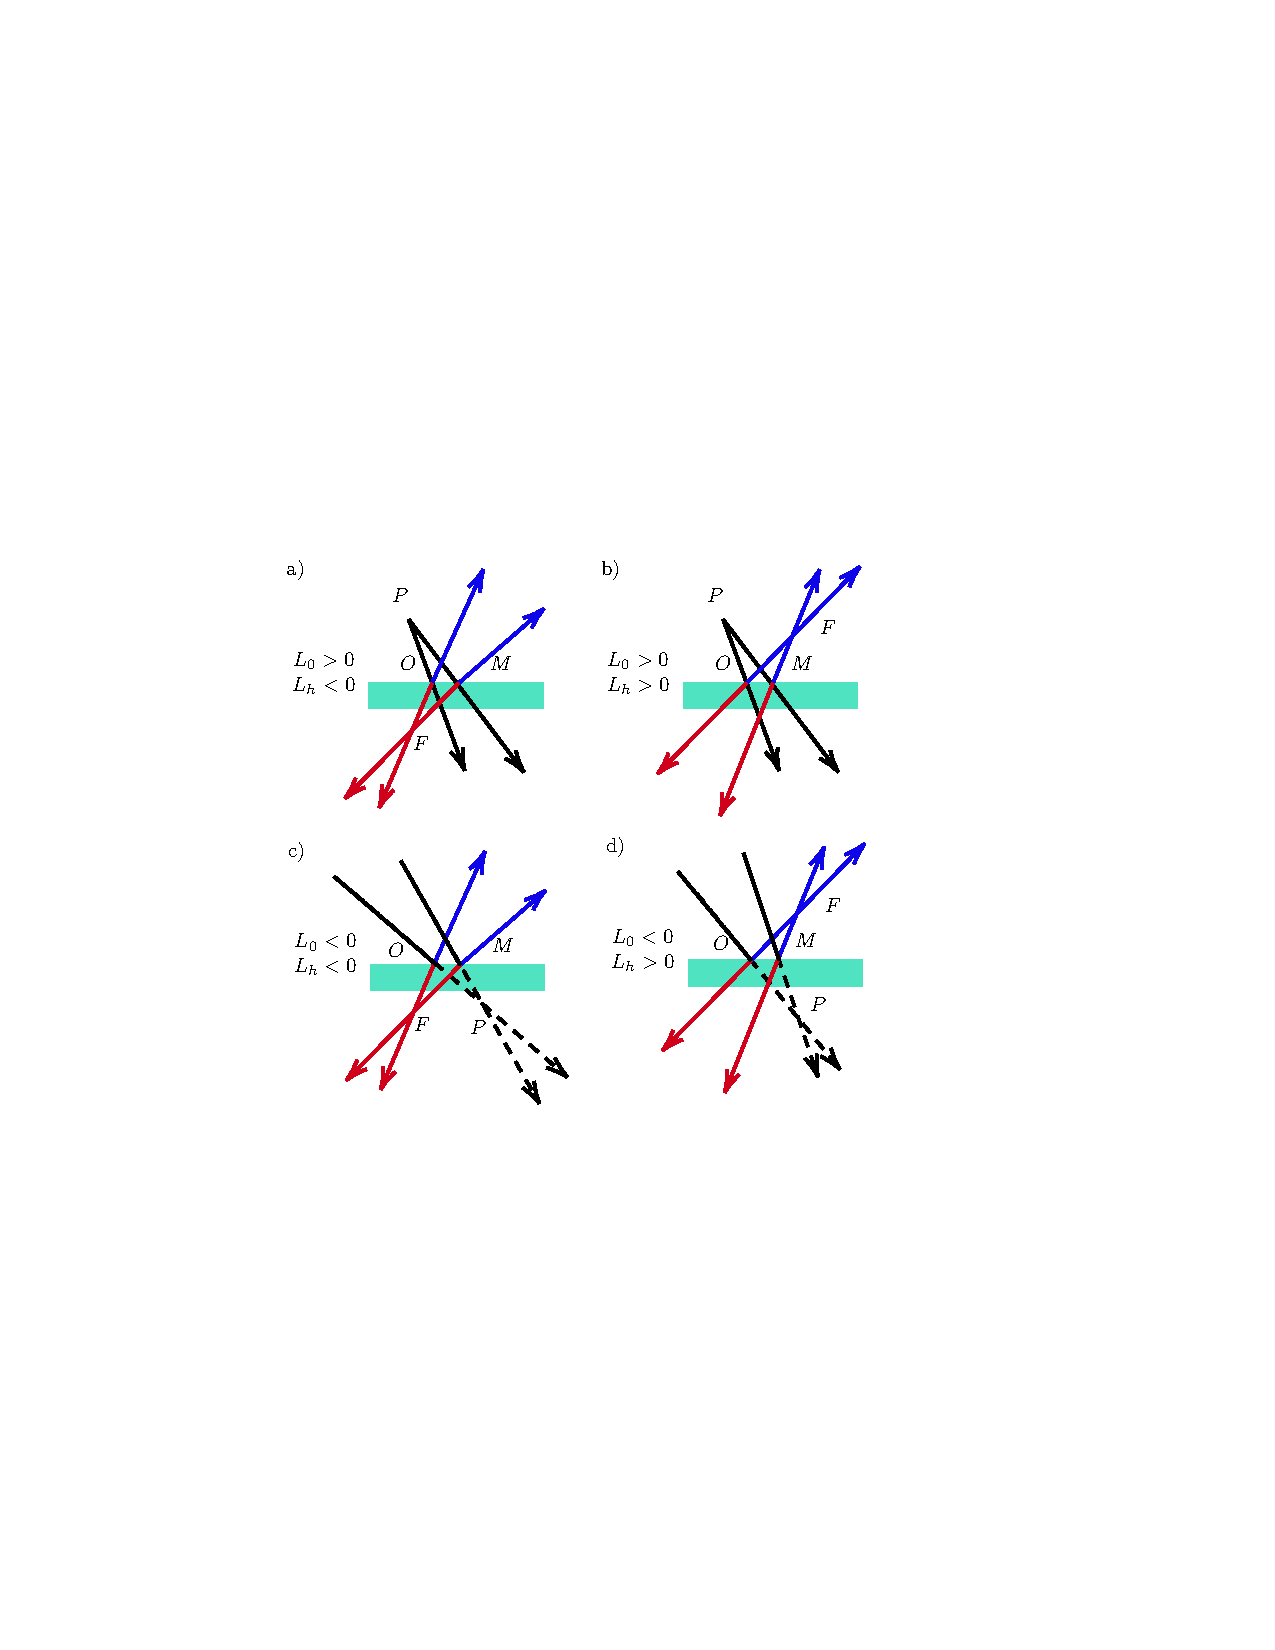
\includegraphics{fig1}
% \end{figure}


\end{document}                    % DO NOT DELETE THIS LINE
%%%%%%%%%%%%%%%%%%%%%%%%%%%%%%%%%%%%%%%%%%%%%%%%%%%%%%%%%%%%%%%%%%%%%%%%%%%%%%
